%%%%%%%%%%%%%%%%%%%%%%%%%%%%%%%%%%%%%%%%%%%%%%%%%%%%%%%%%%%%%%%%%%%%%%%%%%%%%%%%
%2345678901234567890123456789012345678901234567890123456789012345678901234567890
%        1         2         3         4         5         6         7         8

\documentclass[letterpaper, 10 pt, conference]{ieeeconf}  % Comment this line out if you need a4paper

%\documentclass[a4paper, 10pt, conference]{ieeeconf}      % Use this line for a4 paper

\IEEEoverridecommandlockouts                              % This command is only needed if 
                                                          % you want to use the \thanks command

\overrideIEEEmargins                                      % Needed to meet printer requirements.

%In case you encounter the following error:
%Error 1010 The PDF file may be corrupt (unable to open PDF file) OR
%Error 1000 An error occurred while parsing a contents stream. Unable to analyze the PDF file.
%This is a known problem with pdfLaTeX conversion filter. The file cannot be opened with acrobat reader
%Please use one of the alternatives below to circumvent this error by uncommenting one or the other
%\pdfobjcompresslevel=0
%\pdfminorversion=4

% See the \addtolength command later in the file to balance the column lengths
% on the last page of the document

% The following packages can be found on http:\\www.ctan.org
\usepackage{graphics} % for pdf, bitmapped graphics files
\usepackage{epsfig} % for postscript graphics files
\usepackage{mathptmx} % assumes new font selection scheme installed
\usepackage{times} % assumes new font selection scheme installed
\usepackage{amsmath} % assumes amsmath package installed
\usepackage{amssymb}  % assumes amsmath package installed
%\usepackage{xfrac}
\usepackage{graphicx}
\usepackage{makecell}
\usepackage{caption}
\usepackage{mathrsfs}
\usepackage[ruled,vlined]{algorithm2e}
\usepackage[font={small}]{caption}
\usepackage[mathscr]{euscript}
\usepackage{bm}
\usepackage{pifont}% http://ctan.org/pkg/pifont
\usepackage{siunitx}

\usepackage{array}
\newcommand{\PreserveBackslash}[1]{\let\temp=\\#1\let\\=\temp}
\newcommand{\cmark}{\ding{51}}
\newcommand{\xmark}{\ding{55}}
\newcolumntype{C}[1]{>{\PreserveBackslash\centering}p{#1}}
\newcolumntype{R}[1]{>{\PreserveBackslash\raggedleft}p{#1}}
\newcolumntype{L}[1]{>{\PreserveBackslash\raggedright}p{#1}}

% \usepackage{tabularx}

\usepackage[hidelinks]{hyperref}
\hypersetup{
    colorlinks=true,
    linkcolor=blue,
    urlcolor=blue,
    citecolor=blue
}

\usepackage{balance}

\usepackage[utf8]{inputenc}
\usepackage[english]{babel}
\usepackage[backend=biber,sorting=none,citestyle=numeric-comp]{biblatex}
% \usepackage[comma,numbers]{natbib}

\addbibresource{bibliography.bib}
\renewcommand*{\bibfont}{\footnotesize}

% Title
\title{\LARGE \bf

% A Direct Teleoperation Method for Generating Humanoid Multi-Contact Trajectories
% Intuitive Generation of Deployable Humanoid Multi-Contact Trajectories
% An Intuitive Framework for Generating Humanoid Multi-Contact Trajectories

% A Virtual-Reality Driven Approach for Generating Humanoid Multi-Contact Trajectories

Generating Humanoid Multi-Contact through Feasibility Visualization

}

\author{Stephen McCrory$^{1,2}$, Sylvain Bertrand$^{1}$, Achintya Mohan$^{3}$, Duncan Calvert$^{1,2}$, Jerry Pratt$^{4}$, Robert Griffin$^{1,2}$ % <-this % stops a space
\thanks{This work was supported through ONR Grant No. N00014-19-1-2023 and NASA Grant No. 80NSSC20M0197.}%
\thanks{$^{1}$Author is with the Institute of Human and Machine Cognition (IHMC),
        40 S Alcaniz St, Pensacola, FL 32502, USA}% <-this % stops a space
\thanks{$^{2}$Author is with the University of West Florida (UWF),
        11000 University Pkwy, Pensacola, FL 32514, USA}%
\thanks{$^{3}$ Author is with Georgia Institute of Technology, North Avenue Atlanta, GA 30332, USA}%
\thanks{$^{4}$ Author is with Figure AI, Inc., Sunnyvale, CA}%
\thanks{Email: {\tt\small \{smccrory, sbertrand, dcalvert, jpratt, rgriffin\}@ihmc.org, achintya@gatech.edu}}
}

\begin{document}
\maketitle
\thispagestyle{empty}
\pagestyle{empty}

%%%%%%%%%%%%%%%%%%%%%%%%%%%%%%%%%%%%%%%%%%%%%%%%%%%%%%%%%%%%%%%%%%%%%%%%%%%%%%%%
\begin{abstract}

We present a feasibility-driven teleoperation framework designed to generate humanoid multi-contact maneuvers for use in unstructured environments. Our framework is designed for motions with arbitrary contact modes and postures. The operator configures a pre-execution preview robot through contact points and kinematic tasks. A fast estimation of the preview robot’s quasi-static feasibility is performed by checking contact stability and collisions along an interpolated trajectory. A visualization of Center of Mass (CoM) stability margin, based on friction and actuation constraints, is displayed and can be previewed if the operator chooses to add or remove contacts. Contact points can be placed anywhere on a mesh approximation of the robot surface, enabling motions with knee or forearm contacts. We demonstrate our approach in simulation and hardware on a NASA Valkyrie humanoid, focusing on multi-contact trajectories which are challenging to generate autonomously or through alternative teleoperation approaches.

\end{abstract}
%%%%%%%%%%%%%%%%%%%%%%%%%%%%%%%%%%%%%%%%%%%%%%%%%%%%%%%%%%%%%%%%%%%%%%%%%%%%%%%%

% \begin{figure}[t]
%     % \begin{subfigure}{1\linewidth}
%     %   \centering
%     % %   \includegraphics[width=1\linewidth]{figs/fig_1_moti_textattn.pdf}  
%     % %   \includegraphics[width=1\linewidth]{figs/fig_1_moti_textattn_v2.pdf}  
%     %   \includegraphics[width=1\linewidth]{figs/fig_1_moti_textattn_v5.pdf}  
%     %   \vspace{-0.5cm}
%     %     \caption{Amount of attention added to each video clip from the source video and query text in the self-attention layers of Moment-DETR encoder.}
%     %     % \caption{Distribution of attention for source and query in Moment-DETR encoder}
%     %     % Visualization of video clip's self-attention score in Moment-DETR encoder.
%     %   \label{fig:fig1_text_attn_ex}
%     % \end{subfigure}%\hfill% or  or \hspace{0.3\textwidth}
%     \vspace{0.2cm}
%     % \begin{subfigure}{1\linewidth}
%       \centering
%     %   \includegraphics[width=1\linewidth]{figs/fig1_moti_negattn.pdf}  
%       \includegraphics[width=1\linewidth]{figs/fig1_moti_negattn_v3.pdf}  
%       \vspace{-0.4cm}
%     %   \caption{Correspondence of saliency scores on the relevance between video clips and the text query.}
%     % \caption{Predicted saliency scores against the video relevant positive query and video irrelevant negative query}
%       \label{fig:fig1_neg_attn_ex}
%     % \end{subfigure}%\hfill% or  or \hspace{0.3\textwidth}
%     \caption{
%     % 원준 원본
%     % (a) Comparison between attention scores of source and query for each video clip~(We sum the attention scores from video and text). 
%     % We observe that the attention scores are dominated by other clips in the source video. 
%     % Text queries do not account for much attention regardless of the relevance to the video clips.
%     % \textbf{(a)} Inspection of the query dependency in Moment-DETR encoder.
%     % % We visualize the attention score of video tokens in the transformer encoder and observe that text query accounts for only a low portion of attention.
%     % % This tendency occurs regardless of the relevance between the text query and video clips. 
%     % We visualize the attention score of video tokens in the transformer encoder and observe 1) text query only accounts for a low portion of attention, and 2) relevance between video-query pair does not affect the attention scores ratio of text.
%     \textbf{(b)} Comparison of highlight-ness when relevant and non-relevant queries are input.
%     As observed in , existing work only uses queries to play an insignificant role, thereby may not be capable of detecting false queries and considering the video-query relevance even when the problem in (a) is resolved. 
%     % \SE{} % 이 부분이 "not capable of" 란 용어가 세다는 피드백이 있는 듯 합니다. 이러한 능력이 없다는 것은 굉장히 강한 어조인거 같기는 하고, 이러한 경우들이 종종 있다거나 좀 약화시킬 필요가 있어보이긴 하네요.
%     On the other hand, our QD-DETR yields a query-dependent representation that the relevance between the source video and query text is updated in the saliency scores.
%     There is a large gap between positive and negative saliency scores, and scores are consistent since the clips are all highly correlated to others.
%     }
%     \label{fig:motivation_ex}
%     % \captionsetup{belowskip=13pt}
%     % \setlength{\belowcaptionskip}{-10pt}
% \end{figure}
\begin{figure}
    \centering
    \includegraphics[width=1\linewidth]{figs/fig1_moti_negattn_1111.pdf}
    % \includegraphics[width=1\linewidth]{figs/fig1_moti_negattn_1109.pdf}
    % \includegraphics[width=1\linewidth]{figs/fig1_moti_negattn_stat.pdf}
    \vspace{-0.6cm}
    \caption{
        % \SE{} % 수정 필요
        Comparison of highlight-ness~(saliency score) when relevant and non-relevant queries are given.
        We found that the existing work only uses queries to play an insignificant role, thereby may not be capable of detecting negative queries and video-query relevance; saliency scores for clips in ground-truth~(GT) moments are low and equivalent for positive and negative queries.
        % This also results in mispredicted moments when ground-truth~(GT) moment is dominated by clips unrelated to GT since their prediction is highly focused on the video.
        % \SE{} % 여기 한번 더 보면 좋을 듯 합니다. GT moment에 unrelated한 clip이 많으면? label이 틀렷을 경우를 말씀하시는건지?
        % As observed in saliency graph, existing work only uses queries to play an insignificant role, thereby may not be capable of detecting false queries and considering the video-query relevance.
        On the other hand, query-dependent representations of QD-DETR result in corresponding saliency scores to the video-query relevance and precisely localized moments.
        % On the other hand, our QD-DETR yields a query-dependent representation that the
        % saliency scores are in accordance with the relevance between the video and query.
        % text is in accordance with the saliency scores.
        % There is a large gap between positive and negative saliency scores, and scores are consistent since the clips are all highly correlated to others.
}
    \label{fig:motivation_ex}
\end{figure}


\section{Introduction}
% 원준 원본
% Along with the advance of digital devices and platforms, video is now one of the most desired data type for consumers. However, although the large information capacity of videos may be beneficial in many aspects, e.g., informative and entertaining, on the contrary perspective, videos are time-consuming, and hard to search for desirable moments. 
% This has led many creators to use extra manpower to crop and edit the video to generate highlight clips to gain the consumer’s attention.
Along with the advance of digital devices and platforms, video is now one of the most desired data types for consumers~\cite{apostolidis2021video,wu2017deep}.
% SE: Video aware deep learning application & survey papers?
Although the large information capacity of videos might be beneficial in many aspects, e.g., informative and entertaining, inspecting the videos is time-consuming, so that it is hard to capture the desired moments~\cite{anne2017localizing,apostolidis2021video}. 
% This has led many creators to use extra manpower to crop and edit the video to generate highlight clips to gain the consumer’s attention.


% On the other side, 
Indeed, the need to retrieve user-requested or highlight moments within videos is greatly raised.
Numerous research efforts were put into the search for the requested moments in the video~\cite{anne2017localizing, gao2017tall, liu2015multi, escorcia2019temporal} and summarizing the video highlights~\cite{zhang2016video, mahasseni2017unsupervised, badamdorj2022contrastive, wei2022learning}.
% Numerous research efforts were put into the search for the requested moments in the video~\cite{anne2017localizing, gao2017tall, liu2015multi, escorcia2019temporal}, summarizing the video to generate highlights was another popular topic~\cite{zhang2016video, mahasseni2017unsupervised, badamdorj2022contrastive, wei2022learning}.
Recently, Moment-DETR~\cite{momentdetr} further spotlighted the topic by proposing a QVHighlights dataset that enables the model to perform both tasks, retrieving the moments with their highlight-ness, simultaneously.

% 원준 원본
% To detect the desired moments, previous works employed transformer encoder-decoder architectural designs to fuse the text query into the video representations. Moment-DETR~\cite{mDETR} modified detection transformer to process capture the moment as a set, and UMT~\cite{umt} implemented transformer decoder as to output clip-wise saliency. 
% Yet to their outstanding breakthroughs in the literature of moment retrieval with the seminal architectures, their limitation is that the role of the given text query is insignificant in representing the query-conditioned video representation; the attention mechanism of moment DETR is not explicitly conditioned on the text query, and the text query is conditioned on multi-modal clips where the differences between the clips are smoothed after encoding process in UMT.



% \begin{figure}[t]
% \centering
%     \begin{subfigure}[l]{0.37\linewidth}
%       \centering
%       \vspace{0.20cm}
%     %   \includegraphics[width=1\linewidth]{figs/fig_1_moti_textattn.pdf}  
%     %   \includegraphics[width=1\linewidth]{figs/fig_1_moti_textattn_v2.pdf}  
%       \includegraphics[width=1\linewidth]{figs/fig1_moti_violin_a.pdf}  
%       \vspace{-0.60cm}
%     %   \caption{text attention}
%         \caption{Importance of queries in video representation}
%       \label{fig:fig1_text_attn}
%     \end{subfigure}%\hfill% or  or \hspace{0.3\textwidth}
%     \vspace{0.2cm}
%     \begin{subfigure}[r]{0.61\linewidth}
%       \centering
%     %   \includegraphics[width=1\linewidth]{figs/fig1_moti_negattn.pdf}  
%       \includegraphics[width=1\linewidth]{figs/fig1_moti_violin_b.pdf}  
%     %   \caption{neg attention}
%         % \caption{Relation between the highlight-ness and the relevance between videos and query texts.}
%         \caption{Highlight-ness~(saliency) histogram of positive and negative video-query pairs\SE{}}
%       \label{fig:fig1_neg_attn}
%     \end{subfigure}%\hfill% or  or \hspace{0.3\textwidth}
%     % \vspace{-0.2cm}
%     \caption{Overall statistics for attention scores in Fig.~\ref{fig:motivation_ex} in QVHighlights dataset. 
%     (a) For the attention scores that measure how much the text query is generally involved in video representation, we use violin plots to show the probability density. We plot the score for each layer in the encoder.
%     % (b) Using the histogram, we compare how the baseline and QD-DETR yield different salient scores given the positive and negative video-text pairs.
%     (b) Saliency histogram shows the distributional gap between positive and negative video-text query pairs of baseline~(Moment-DETR) and proposed QD-DETR.\SE{}
%     }
%     \label{fig:motivation}
%     % \captionsetup{belowskip=13pt}
%     % \setlength{\belowcaptionskip}{-10pt}
% \end{figure}

% \begin{figure}[t]
% \centering

%     \begin{subfigure}[r]{1\linewidth}
%       \centering
%       \hspace{-0.2cm}
%     %   \includegraphics[width=1\linewidth]{figs/fig1_moti_negattn.pdf}  
%       \includegraphics[width=1.1\linewidth]{figs/fig1_moti_violin_a_v2.pdf}  
%     %   \caption{neg attention}
%         % \caption{Relation between the highlight-ness and the relevance between videos and query texts.}
%         \vspace{-0.5cm}
%         % \caption{Saliency histogram of positive and negative video-query pairs}
%         \caption{We plot the histograms and its average value~(dotted line) to compare saliency scores when true and false text queries are given for each method. (left) Since the video representations do not include much textual information, both the true and false queries yield similar saliency scores. (Middle) Even when the video representation is enforced to be updated with the textual information, the issue is not much resolved. (Right) By extracting discriminative features in the text query, distributions are differentiated.
%         % \SE{} % R1@0.5 설명
%         Also, R1@0.5 indicates evaluation metric, Recall at 1 with IoU 0.5 threshold on QVhighlight \textit{val} set.
%         }
%       \label{fig:fig1_neg_attn}
%     \end{subfigure}%\hfill% or  or \hspace{0.3\textwidth}
%     \\
%     \begin{tabular}{cc}
%     \hspace{-0.2cm}
%         \begin{minipage}{.4\linewidth}
%             \begin{subfigure}[l]{1\linewidth}
%               \centering
%             %   \vspace{0.20cm}
%             %   \includegraphics[width=1\linewidth]{figs/fig_1_moti_textattn.pdf}  
%             %   \includegraphics[width=1\linewidth]{figs/fig_1_moti_textattn_v2.pdf}  
%               \includegraphics[width=1\linewidth]{figs/fig1_moti_violin_a.pdf}  
%               \vspace{-0.60cm}
%             %   \caption{text attention}
%                 \caption{Importance of queries in video representation}
%               \label{fig:fig1_text_attn}
%             \end{subfigure}%\hfill% or  or \hspace{0.3\textwidth}
%         \end{minipage}
        
%         \begin{minipage}{.6\linewidth}
%             \vspace{-0.2cm}
%             \caption{Overall statistics of Fig.~\ref{fig:motivation_ex} in QVHighlights dataset. 
%             (a) Saliency histogram shows the distributional gap between positive and negative video-text query pairs.
%             % (a) For the attention scores that measure how much the text query is generally involved in video representation, we use violin plots to show the probability density. We plot the score for each layer in the encoder.
%             % (b) Using the histogram, we compare how the baseline and QD-DETR yield different salient scores given the positive and negative video-text pairs.
%             % (b) Text ratio in self-attention layer to  of Moment-DETR
%             % (b) Ratio of text when representing video tokens in self-attention of Moment-DETR.
%             % (b) Magnitude of attention text query involved.
%             % (b) Attention score of video tokens
%             % (b) Magnitude of text query to refine the video tokens in self-attention layer of Moment-DETR.
%             (b) Probability density depicting the weight of the text query in attention score for video clips. Scores are from the self-attention layers in Moment-DETR encoder.
%             % (b) The text query ratio in attention score of video clips (Self-attention layer in Moment-DETR encoder). We use violin plots to show probability density.
%             % 텍스트 쿼리가, 비디오 피쳐에 얼만큼 attend 하는지
%             }
%         \end{minipage}
    
%     \end{tabular}
%     \vspace{-0.5cm}
%     \label{fig:moti}
%     % \captionsetup{belowskip=13pt}
%     % \setlength{\belowcaptionskip}{-10pt}
% \end{figure}


% \begin{figure}
%     \centering
%     % \includegraphics[width=1\linewidth]{figs/fig1_moti_negattn_1109.pdf}
%     \includegraphics[width=1\linewidth]{figs/fig1_moti_negattn_stat_v2.pdf}
%     \vspace{-0.8cm}
%     \caption{
%         Histogram of saliency when the positive and negative queries are given. We plot the histograms and its average value~(dotted line) to compare saliency scores when relevant~(positive) and irrelevant~(negative) text queries are given for each method. (Left) Since the video representations do not properly reflect textual information, both the positive and negative queries yield similar saliency scores. 
%         % (Middle) Even when the video representation is enforced to be updated with the textual information, the issue is not much resolved. 
%         (Right) By representing video clips in query-dependent manner, distributions are differentiated.
%     }
%     \vspace{-0.6cm}
%     \label{fig:motivation}
% \end{figure}


% One of the demanding task is moment retrieval task, which is detecting the desired moments from the given query, typically the text query.
When describing the moment, one of the most favored types of query is the natural language sentence~(text)\cite{anne2017localizing}. 
While early methods utilized convolution networks~\cite{zhang2020learning, gao2021fast, wang2020temporally}, recent approaches have shown that deploying the attention mechanism of transformer architecture is more effective to fuse the text query into the video representation.
% To handle these modalities, previous works simply employed the attention mechanism of transformer architecture to fuse the text query into the video representation.
For example, Moment-DETR~\cite{momentdetr} introduced the transformer architecture which processes both text and video tokens as input by modifying the detection transformer~(DETR), and UMT~\cite{umt} proposed transformer architectures to take multi-modal sources, e.g., video and audio. 
Also, they utilized the text queries in the transformer decoder.
Although they brought breakthroughs in the field of MR/HD with seminal architectures, they overlooked the role of the text query.
To validate our claim, we investigate the Moment-DETR~\cite{momentdetr} in terms of the impact of text query in MR/HD~(Fig.\ref{fig:motivation_ex}).
Given the video clips with a relevant positive query and an irrelevant negative query, we observe that the baseline often neglects the given text query when estimating the query-relevance scores, i.e., saliency scores, for each video clip.
% the output saliency score, i.e. query-relevance scores.
% Based on the observation, we traced the actual saliency prediction of the model against both the video-relevant query and the irrelevant dummy one where we find that the baseline often neglects the given text query when estimating the query-relevance scores of video clips.
% For example, in Fig.~\ref{fig:motivation_ex}, saliency scores are not affected even when the query is substituted with the dummy.
% % General statistics for Fig.~\ref{fig:motivation_ex} is shown in Fig.~\ref{fig:motivation}. 
% General statistics corresponding to Fig.~\ref{fig:motivation_ex} are also shown in Fig.~\ref{fig:motivation}.



% The limitation of the concrete baseline~\cite{momentdetr} is inspected in two different aspects; 1) Utilization of text-query in the encoding process and 2) the output saliency score, i.e. query-relevance scores.
% Firstly, we visualize the attention score when video clips are given as a query in self-attention. 
% We observe that the text queries have relatively small impacts compared to other video features, as shown in Fig.~\ref{fig:fig1_text_attn_ex}.
% That is, the text does not account for much in representing every video clip, although the goal of MR/HD is to detect query-relevant moments.
% Based on the observation, we traced the actual saliency prediction of the model against both the video-relevant query and the irrelevant dummy one where we find that the baseline often neglects the given text query when estimating the query-relevance scores of video clips.
% For example, in Fig.~\ref{fig:motivation_ex}, saliency scores are not affected even when the query is substituted with the dummy.
% % General statistics for Fig.~\ref{fig:motivation_ex} is shown in Fig.~\ref{fig:motivation}. 
% General statistics are also shown in Fig.~\ref{fig:motivation}.

% Consequently, in Fig.~\ref{fig:fig1_neg_attn_ex}~(b), we found that the baseline often neglects the given text query when estimating the query-relevance scores of video clips; 
% For example, 


% We validate the previous work sometimes neglects the given query when estimating the saliency of video clips.
% For example, there is an example that the saliency scores from positive and negative queries cannot be distinguishable, as shown in Fig.~\ref{fig:fig1_neg_attn_ex}.
% % 우리는 추가로 text attention을 추가도 해봤지만, 효과가 있긴 했으나, still 이슈가 있는 것을 확인하였다?
% % Still, we observe that assuring the high attendance of text queries does not resolve the overlap which motivates us to question the quality of the naive use of task-agnostic text representation~\cite{momentdetr, umt}.
% We found that introducing the text-attention for ensuring the high attendance of text queries relieve the overlap, but there still be a severe overlap.


% To validate their limitations, we inspect the impacts of text queries in the concrete baseline~\cite{momentdetr} with the two different aspects, 1) tendency of attention in self-attention layer and 2) saliency score, i.e. query-relevance scores. \SE{} % attention 이 갑자기 등장하는가?
% Firstly, we visualize the attention score when video clips are given as a query in self-attention. We observe the text queries have relatively low attention scores compared to the video features, as shown in Fig.~\ref{fig:fig1_text_attn_ex}.
% That is, the text does not account for much in representing every video clip, although the goal of MR/HD is to detect query-relevant moments.
% Based on this observation, we trace the actual saliency prediction of the model against both positive and negative text queries.
% We validate the previous work sometimes neglects the given query when estimating the saliency of video clips.
% For example, there is an example that the saliency scores from positive and negative queries cannot be distinguishable, as shown in Fig.~\ref{fig:fig1_neg_attn_ex}.
% % 우리는 추가로 text attention을 추가도 해봤지만, 효과가 있긴 했으나, still 이슈가 있는 것을 확인하였다?
% % Still, we observe that assuring the high attendance of text queries does not resolve the overlap which motivates us to question the quality of the naive use of task-agnostic text representation~\cite{momentdetr, umt}.
% We found that introducing the text-attention for ensuring the high attendance of text queries relieve the overlap, but there still be a severe overlap.



% Thus, we 
% query dependency를 높이기 위해 
% Cross-attention? text-attention? detailed explanation on text-attention should be needed?
% By handling these two issues, we find that more precise retrieval can be achieved.
% 
% 
%
% By projecting video-discriminative text features with high text attendance to source video, we f 
% We also find the need to improve the quality of query features since assuring high text attendance also results in...
% pairs are not finetuned to be discriminative that even the similarity within the pairs does not reflect the relevance between the query and the video clips.
% General statistics for Fig.~\ref{fig:motivation_ex} is shown in Fig.~\ref{fig:motivation}. 
% \SE{} % 이거 ??로 뜨는데, 위처럼 figure 그리면 label이 안되는걸까요
% \SE{}
% 형님 아래 사항 생각 좀 해보는게 좋을 거 같아요.
% fig 1. (a) 그림만 봤을 때 모든 clip에 대해 text attention이 일정이상 존재하긴 하니까, 뭔가 not assured to be conditioned가 와닿지 않는거 같아요.
% + 왜 text가 항상 attend 해야하나?
% not assured to be conditioned --> text shows relatively low affects compared to video 같이 실제 나타난 현상까지 같이 적으면 어떨까 싶어요.
% fig 1. (b) 덜 반영한다?

% \SU{}
% 일단 text가 attend 잘 되어야 한다는 것에 좀 궁금점이 생깁니다. 결국에는 text와 관련있는 frame들을 attend해서 higlight를 찾아야 하는게 아닐까요? 그리고, 현제 저희의 모델 구조상 text query가 Key와 Value로 거의 활용되고 있는데 그렇다면 결국에는 해당 모델은 text에 대한 attention이 전혀 없다고 봐도 무방하지 않을까요? 그런 면에서 text attention을 강조하는게 좀 걸리긴 합니다.

% Specifically, the text query is not assured to be explicitly conditioned on every clip of the video, and as the query texts are evenly treated, discriminative keywords may not be spotlighted.
% attention mechanism of Moment-DETR is not explicitly conditioned on the text query as shown in Fig~\ref{}(d), and in UMT, the text are only used for conditioning the queries while the video representation are refined itself by self-attention.

% \begin{figure}[t]
%     \begin{subfigure}{1\linewidth}
%       \centering
%     %   \includegraphics[width=1\linewidth]{figs/fig_1_moti_textattn.pdf}  
%     %   \includegraphics[width=1\linewidth]{figs/fig_1_moti_textattn_v2.pdf}  
%       \includegraphics[width=1\linewidth]{figs/fig_1_moti_textattn_v4.pdf}  
%       \vspace{-0.5cm}
%     %   \caption{text attention}
%         \caption{Distribution of attention scores in Moment-DETR encoder}
%       \label{fig:fig1_text_attn}
%     \end{subfigure}%\hfill% or  or \hspace{0.3\textwidth}
%     \vspace{0.2cm}
%     \begin{subfigure}{1\linewidth}
%       \centering
%     %   \includegraphics[width=1\linewidth]{figs/fig1_moti_negattn.pdf}  
%       \includegraphics[width=1\linewidth]{figs/fig1_moti_negattn_v2.pdf}  
%       \vspace{-0.5cm}
%     %   \caption{neg attention}
%         \caption{Saliency score against positive and negative text queries}
%       \label{fig:fig1_neg_attn}
%     \end{subfigure}%\hfill% or  or \hspace{0.3\textwidth}
%     \vspace{0.2cm}
%     \begin{subfigure}{1\linewidth}
%       \centering
%     %   \includegraphics[width=1\linewidth]{figs/fig1_moti_violin.pdf}  
%       \includegraphics[width=1\linewidth]{figs/fig1_moti_violin_v2.pdf}  
%       \vspace{-0.5cm}
%       \caption{violin}
%       \label{fig:fig1_violin}
%     \end{subfigure}%\hfill% or  or \hspace{0.3\textwidth}
%     \vspace{-0.2cm}
%     \caption{(a) 1. portion of text attention vs. video attention 2. relation with text query and content (e.g. fg, bg) of clip seems not to affect the attention score
%     (b) 1. high variability even though entire clips are highly correlated with the given text query 2. positive and negative query makes overlaps on saliency score distribution
%     (3) actual distribution on validation dataset.}
%     \label{fig:motivation}
%     % \captionsetup{belowskip=13pt}
%     % \setlength{\belowcaptionskip}{-10pt}
% \end{figure}

To this end, we propose Query-Dependent DETR~(QD-DETR) that produces query-dependent video representation.
% Our key focus is to ensure each clip in predicted moments is explicitly conditioned by the query, particularly on the video-descriptive portion of the text query.
% Our key focus is to ensure that query-relevant clips are predicted by enforcing each clip to be explicitly conditioned by the query.
%Our key focus is to ensure that the model prediction for each clip is highly relevant to the query.
Our key focus is to ensure that the model's prediction for each clip is highly dependent on the query.
% by enforcing each clip to be explicitly conditioned by the query. :)
% hmm...
% \SE {} % "query-relevant clips are predicted" 이 문장이 좀 애매한거 같습니다. relevant 클립을 놓지지 않고 찾는 것을 보장한다? 이런 느낌인지 아니면 높은 saliency 를 주는게 목적이다? model prediction이 query-relevance를 반영하는 것을 보장한다?
% Our key focus is to ensure that the model prediction reflects query-relevance of clips by enforcing each clip to be explicitly conditioned by the query.
First, to fully utilize the contextual information in the query, we revise the transformer encoder to be equipped with cross-attention layers at the very first layers.
% 상익's thought :  single video - query간의 관계만 고려 - 같은 word가 더 많이 쓰이는 것을 보고 
% 교수님's thought : neg pair 를 쓰면 쿼리를 보지 않고서는 video clip간만 고려하는 것이 사라짐. 왜냐면 0으로 내보내야 하기 때문. --> SE: relative difference 만 고려하다가, 
By inserting a video as the query and a text as the key and value of the cross-attention layers, our encoder enforces the engagement of the text query in extracting video representation.
% 원준 교수님 코멘트 반영해서 다시
Then, in order to not only inject a lot of textual information into the video feature but also make it fully exploited, we leverage the negative video-query pairs generated by mixing the original pairs.
Specifically, the model is learned to suppress the saliency scores of such  negative~(irrelevant) pairs.
Our expectation is the increased contribution of the text query in prediction since the videos will be sometimes required to yield high saliency scores and sometimes low ones depending on whether the text query is relevant or not.
% \SE{}
% learns to?
% By suppressing the saliency scores of the irrelevant video-query pairs, the model learns to spotlight only the video-specific discriminative words in the query.
% % \SE{} % ====================== 상익 수정 ========================
% However, this architectural design still lacks the capability of identifying the video-descriptive keywords in the query.
% % However, this architectural design still lacks in identifying proper query relevance.
% This is because the current training scheme only focuses on the interactions of video and clips within a single video while neglecting information shared throughout the entire video.
% % We argue the problem of the current training scheme that only focuses on distinguishing the clips in a single video while neglecting information shared throughout the entire video.
% Therefore, we leverage the negative video-query relationships to enhance the capability of identifying the contextual similarity of query and video clips.
% 
% 원준 원본 
% However, this architectural design heavily relies on the quality of the text query.
% Therefore, we leverage the negative video-query relationships to enable the model to emphasize key corresponding query features.
% By suppressing the saliency scores of the irrelevant video-query pairs, the model learns to spotlight only the video-specific discriminative words in the query.
% =========================================================
Lastly, to apply the dynamic criterion to mark highlights for each instance, we deploy a saliency token to represent the entire video and utilize it as an input-adaptive saliency criterion. 
With all components combined, our QD-DETR produces query-dependent video representation by integrating source and query modalities.
This further allows the use of positional queries~\cite{dabdetr} in the transformer decoder.
% Furthermore, we can exploit the advanced DETR decoder architectures using the positional information, e.g., DAB-DETR, since our encoded tokens consist of identical position representations from a single modality.
% \SE{} % ====================== 상익 수정 ========================
% Furthermore, we can exploit the advanced DETR decoder architectures using the positional information, e.g., DAB-DETR, since our video clip tokens consist of identical position representations from a single modality.
% 원준 원본
% It also enables the use of advanced DETR decoder architectures, e.g., DAB-DETR, for the first time, as these works exploit the position information within a single modality.
% =========================================================
Overall, our superior performances over the existing approaches validate the significance of the role of text query for MR/HD.
% Our extensive experiments on QVHighlights, TVSum, and Charades-STA datasets validate the significance of considering the role and the quality of text query.

% All components combined with dynamic anchor moments for the query of decoder, our FOQUE fosters the query-dependent video representation, thereby making the 
% All components combined, our modified transformer encoding process fosters the query-dependent video representation thereby achieving the state-of-the-art results on various benchmarks of moment-retrieval and highlight detection.
	
% -	Video Platform & Streamer & Consumer의 증가. 
% Video는 다른 데이터 타입보다 정보가 많아 유용하지만, 이는 다른 말로 해석하면 video를 보는 것은 time-consuming 하고, 원하는 것을 찾아보기에는 힘들 수 있음.
% 따라서, 많은 매체에서는 사람들의 더 많은 이목을 끌기 위해 highlight 비디오라는 것을 편집하여 공유도 함.
% 하지만, highlight video를 만들기 위해 사람의 노력이 필요한 현 시점에서, This spotlights the need to retrieve the user-requested / Highlight moments in the video.

% -	이전에도 이러한 문제를 해결하기 위해 (asdfasdf) for moment retrieval, (asdfasdf) for highlight detection 등이 제안 되었지만, 이들은 비디오의 특정 영역을 찾는다는 공통된 목적을 가지고 있으면서도, 데이터 셋의 한계로 인해 따로 연구되었음. 이를 문제 삼으며, 최근에는 두 task를 동시에 학습할 수 있는 dataset이 소개 되었는데, 컴퓨터비전에서 최근 각광을 받고 있는 Transformer 모델 도입과 함께 큰 발전을 거듭하고 있음.

% -	구체적으로, 이 두가지 task를 수행하기 위해서는 transformer를 두가지 방법으로 이용할 수 있는데, moment-DETR 처럼 moment 를 clip의 set 단위로 예측할 수 있고, UMT 처럼 clip-wise prediction을 할 수 있음. 하지만, 이들은 query를 condition이 아닌 video와 동등한 레벨로 취급하거나 [mDETR], 매 클립이 self-attention으로 mixing 된 후에 condition을 걸어주어 clip간의 차이를 확실하지 이용하지 못하였고, 또한, 확실하게 condition으로 주지 못하였고, video와 query 사이의 관계를 한정적으로만 이용하였다.

% -	따라서, we explore three different ways to fully exploit query information. First, we design one-way cross-attention layer to condition every clip with the query features. Then, we utilized the negative video-text pairs to better model the relationships between the video and the text embeddings. Lastly, we define the saliency token to be the video-query dependent saliency estimator.


















% ===================== neg pair 부분 ===========================
% Nevertheless, the current training scheme, only considering the given video-query pair, still disturbs the model from identifying proper query-relevance prediction.
% In detail, the model focus on learning the fine-grained discrepancy between video clips, while neglecting the information they share, which contains significant clues to understand the context of video.
% Therefore, we leverage the negative video-query relationships to enhance the capability of identifying the contextual similarity of query and video clips.
% Therefore, we leverage the negative video-query relationships by suppressing those pairs, so that enhance the capability of identifying the contextual similarity of query and video clips.
% We hypothsize the diversity in query-video pairs are insufficient to learn the general relationship between text query and video.
% Therefore, we leverage the negative video-query relationships by suppressing the saliency scores of the irrelevant video-query pairs.
% However, this architectural design still lacks in identifying proper query relevance.
% We argue that the current training scheme only focuses on learning the fine-grained discrepancy between clips in a single video, while neglecting the information they share, which contains significant clues to understand the context of the video.
% Therefore, we leverage the negative video-query relationships to enhance the capability of identifying the contextual similarity of query and video clips.
% However, this architectural design still lacks in identifying proper query relevance.
% We argue the problem of the current training scheme that only focuses on learning the fine-grained discrepancy between clips in a single video.
% That is, the current design neglects the information shared throughout the video, although it contains significant clues to understand the context of the video.
\section{Related Work}
\label{sec:related_work}
\subsection{Co-Speech Gesture Synthesis}
The early approaches for generating co-speech gestures often involve creating linguistic rules to translate speech input into a sequence of pre-collected gesture segments, which are typically referred to as rule-based methods \cite{cassell1994rulefullbody,cassell2001beat,kipp2004gesture,kopp2006bml}. \citet{wagner2014rulereview} provide a comprehensive review of these methods. Rule-based methods produce interpretable and controllable results, but creating gesture datasets and rules requires significant effort. To alleviate the manual effort of designing rules in rule-based methods, data-driven approaches have gradually become predominant in this field. \citet{nyatsanga2023data_driven_gesture_survey} offer a thorough survey of these methods. Early data-driven approaches aim to directly learn mapping rules from data through statistical models \cite{neff2008videogesture,levine2009prosodygesture,levine2010gesturecontroller} and combine them with predefined gesture units for gesture generation. Later, the powerful modeling capability of deep neural networks makes it possible to train complex end-to-end models using raw speech-gesture data directly. One option is deterministic models, such as MLP \cite{kucherenko2020gesticulator}, CNN \cite{habibie2021videogesture}, RNN \cite{yoon2019robot,yoon2020trimodalgesture,bhattacharya2021affectivegesture,liu2022hierarchicalgesture}, and Transformer \cite{bhattacharya2021text2gestures}. Another choice is generative models, including flow-based models \cite{alexanderson2020stylegesture,ye2022styleflowgesture}, VAEs \cite{li2021audio2gesture,ghorbani2022zeroeggs}, and VQ-VAE \cite{yi2022talkshow,yazdian2022gesture2vec,liu2022vqgesturevideo}. Due to the inherent many-to-many relationship between speech and gesture, end-to-end models can generate natural-looking gestures but face challenges in ensuring content matching between speech and generated gestures \cite{yoon2022genea}. To address this issue, some neural systems aim to explicitly model both rhythm and semantics from the perspective of model structure \cite{kucherenko2021speech2properties2gestures,ao2022rhythmicgesticulator,liu2022disco} or training supervision strategy \cite{liang2022seeg}. Furthermore, hybrid systems, such as the combination of deep features and motion graphs \cite{zhou2022gesturemaster}, have been proposed to harness the advantages of different approaches. Recently, diffusion models \cite{sohldickstein2015diffusion,song2020improvedscore,ho2020ddpm} have demonstrated impressive results in image synthesis \cite{ramesh2022dalle2} and human motion generation \cite{tevet2022humanmotiondiffusion, zhang2022motiondiffuse}. Inspired by these works, our system adapts the latent diffusion model \cite{rombach2022latentdiffusion} for the co-speech gesture generation task and achieves appealing results.

\subsection{Style Control for Human Motion}
A typical approach to style control for human motion involves specifying a motion clip as a reference and transferring the reference clip's style to the source motion. This task is also known as \emph{style transfer}. Early works in motion style transfer integrate traditional machine learning techniques with manually defined features to infer motion styles \cite{hsu2005motion_style_translation,ma2010motion_style_transfer,xia2015realtime_motion_style_transfer,yumer2016spectral_motion_style_transfer}. Recently, deep learning-based methods have significantly enhanced motion quality. \citet{holden2016deepmotion} first propose a learning framework enabling motion style control through optimization in the motion manifold space. \citet{du2019stylemotioncvae} improve transfer efficiency by training a conditional VAE. \citet{mason2018few-shot_motion_style_transfer} use few-shot learning to generate stylized locomotion. \citet{aberman2020adain} employ a temporally invariant adaptive instance normalization (AdaIN) layer for target style injection, eliminating the need for paired data during training. \citet{wen2021stylemotionflow} achieve unsupervised style transfer using a flow model. \citet{jang2022motionpuzzle} introduce a method capable of controlling styles for individual body parts.

Previous co-speech gesture synthesis systems with style control can be categorized based on whether or not they require style labels. For methods needing labeled data, early works can only learn an individual style for one generator \cite{levine2010gesturecontroller,neff2008videogesture,ginosar2019stylegesture}. \citet{ahuja2022lowresource} propose a strategy that efficiently adapts the source generator to another speaker style using low-resource data. Some works learn a speaker style embedding space with labeled speaker-motion data, enabling gesture style control by sampling from this space \cite{ahuja2020stylegesture,yoon2020trimodalgesture,bhattacharya2021affectivegesture}. \citet{alexanderson2020stylegesture} aimat controlling fine-grained styles, such as gesturing speed and spatial scope, using preprocessed control signal-motion data. Their later work \cite{alexanderson2022diffusiongesture} utilizes a diffusion model for audio-driven motion synthesis, achieving label-based style control by training the model on labeled data. For methods not requiring style labels, \citet{habibie2022motionmatching} propose a motion matching framework to achieve flexible style control. Other studies achieve arbitrary style control by imitating an example given as a video \cite{liu2022hierarchicalgesture} or a motion clip \cite{ghorbani2022zeroeggs,ye2022styleflowgesture,kuriyama2022tokenizedgestures}.  In this work, we utilize a CLIP-based encoder to extract a style embedding from an arbitrary text prompt and incorporate it into the generator via an AdaIN layer, guiding the synthesis of stylized gestures. Our system supports fine-grained multimodal style prompts as opposed to label-based style control. It employs a self-supervised learning scheme and eliminates the need for labeled data. Additionally, we use an autoregressive model rather than a parallel model, making it potentially suitable for real-time applications.
\section{A Fine-grained Evaluation Framework}
This section defines the keyphrase evaluation problem and proposes a multi-dimensional evaluation framework. We then introduce the metrics to evaluate each of the dimensions, including (1) semantic-based matching for saliency and coverage, (2) lexical and semantic overlap for diversity, (3) retrieval-based evaluation for utility, and (4) model-based evaluation for naturalness and faithfulness.

\subsection{Problem Formulation}
The \textit{keyphrase evaluation} problem for a single document can be formulated with a 4-element tuple $(\mathcal{X}, \mathcal{Y}, \mathcal{P}, \mathcal{C})$. $\mathcal{X}$ is the input document. $\mathcal{Y}=\{y_1,...,y_n\}$ is a list of $n$ reference phrases written by human. $\mathcal{P}=\{p_1,...,p_m\}$ is a list of $m$ predictions made by a model $\mathcal{M}$ on $\mathcal{X}$. To focus on semantic-based evaluation, we do not differentiate between keyphrases that appear in $\mathcal{X}$ ("present keyphrases") and those that do not ("absent keyphrases").  As the definition of keyphrases is domain-dependent, we introduce $\mathcal{C}$, a set of corpus documents, to represent the domain.

A \textit{keyphrase metric} is a function $f$ whose value $f(\mathcal{X}, \mathcal{Y}, \mathcal{P}, \mathcal{C})\in\mathbb{R}$ reflects a certain quality of $\mathcal{M}$. $f$ is a phrase-level metric if it is calculated as the average of metric values calculated on each $p_i\in\mathcal{P}$. $f$ is reference-free if its calculation is independent of $\mathcal{Y}$, or reference-based otherwise. In practice, the final score for $\mathcal{M}$ is often the averaged score over a set of testing documents. 

\subsection{How to define a good keyphrase system?}
Deciding the evaluation goals is crucial for building evaluation systems. We argue that the following six unique properties should be considered when evaluating keyphrase exaction or generation systems:

\begin{compactenum}
    \item \textbf{\textit{Naturalness}}: $p_i$ is a natural and grammatically correct phrase.
    \item \textbf{\textit{Faithfulness}}: all keyphrases in $\mathcal{P}$ are covered in $\mathcal{X}$, i.e., free of hallucination.
    \item \textbf{\textit{Saliency}}: $p_i$ carries salient information associated with $\mathcal{X}$. As the saliency varies with the domain, we use $\mathcal{Y}$ as a proxy for the set of salient information associated with $\mathcal{X}$.
    \item \textbf{\textit{Coverage}}: how much salient information in $\mathcal{X}$ is covered by $\mathcal{P}$.
    \item \textbf{\textit{Diversity}}: the degree to which $\mathcal{P}$ contains diverse concepts with minimal repetition.
    \item \textbf{\textit{Utility}}: the extent to which $\mathcal{P}$ facilitates downstream applications, such as retrieval.
\end{compactenum}

Table \ref{tab:kp-sys-property-assumptions} outlines the assumptions of these properties. Naturalness, faithfulness, and saliency are targeted at evaluating individual phrases, while coverage, diversity, and utility evaluate the entire set $\mathcal{P}$. Faithfulness and utility require $\mathcal{X}$, while saliency and coverage require $\mathcal{Y}$. To gauge the utility, $\mathcal{C}$ is required for specifying the domain. Next, we discuss how we operationalize these dimensions.


\subsection{Saliency and Coverage}
\fcolorbox{pink}{pink}{\parbox{0.47\textwidth}{
\textit{\textbf{Desiderata}: semantically similar phrases should be credited; matching should be at phrase level.}}
}
\vspace{0.3pt}

Precision and recall with exact matching can capture saliency and coverage, while they struggle at dealing with semantic similarity. Conversely, BertScore \citep{bert-score} calculated with concatenated predictions and references captures semantic similarity, but its token-wise matching with contextual representations built in one encoding pass prevents evaluating the semantic similarity among individual phrases. To enjoy the advantage of both, we introduce \textit{phrase-level semantic-based} matching and define semantic precision ($SemP$), recall ($SemR$), and F1 ($SemF1$) as follows:
\begin{equation}
\resizebox{0.9\hsize}{!}{$SemP(\mathcal{P},\mathcal{Y})=\frac{\sum_{p\in\mathcal{P}}\max_{y\in\mathcal{Y}}(\mathbbm{1}(sim(p,y)>\alpha)\cdot sim(p,y))}{|\mathcal{P}|}$}\nonumber
\end{equation}
\begin{equation}
\resizebox{0.9\hsize}{!}{$SemR(\mathcal{P},\mathcal{Y})=\frac{\sum_{y\in\mathcal{Y}}\max_{p\in\mathcal{P}}(\mathbbm{1}(sim(p,y)>\alpha)\cdot sim(p,y))}{|\mathcal{Y}|}$}\nonumber
\end{equation}
\begin{equation}
\resizebox{0.75\hsize}{!}{$SemF1(\mathcal{P},\mathcal{Y})=\frac{2\cdot SemP(\mathcal{P},\mathcal{Y})\cdot SemR(\mathcal{P},\mathcal{Y})}{SemP(\mathcal{P},\mathcal{Y}) + SemR(\mathcal{P},\mathcal{Y})}$}\nonumber
\end{equation}
where $sim$ is a function defining the similarity between the representation of two phrases and $\alpha$ is a hyperparameter to filter out the noise in $sim$\footnote{We use 
$\alpha=0$ throughout the paper. $\alpha$ is included in the formulation to satisfy application-specific needs.}. To quantify whether $\mathcal{P}$ covers the overall semantics of $\mathcal{Y}$, we also introduce an overall semantic coverage index $SemCov$, defined as 
\begin{equation}
\resizebox{0.9\hsize}{!}{$SemCov(\mathcal{P}, \mathcal{Y})=sim(union(\mathcal{P}), union(\mathcal{Y}))$}\nonumber
\end{equation}
where $union$ is a function that computes a representation for a set of phrases.


\setlength{\tabcolsep}{3pt}
\begin{table}
    \centering
    \resizebox{\linewidth}{!}{%
    \begin{tabular}{l | c c c c}
    \hline
     & \texttt{KP-Set} & \texttt{Input} & \texttt{Reference} & \texttt{Corpus}  \\
    \hline
    \textbf{{Reference Agreement}} & \cmark &  & \cmark &  \\
    \textbf{{Faithfulness}} &  & \cmark &  &  \\
    \textbf{{Diversity}} & \cmark &  &  &  \\
    \textbf{{Utility}} & \cmark & \cmark &  & \cmark \\
    \hline
    \end{tabular}
    }
    \vspace{-2mm}
    \caption{Assumptions of \textsc{KPEval}'s aspects: whether they operate on a set of keyphrases (\texttt{KP-Set}) and whether they require input, reference, or a corpus.}
    \label{tab:kp-sys-property-assumptions}
    \vspace{-4mm}
\end{table}

To define the metrics, the key ingredient is the $sim$ function, which encodes two phrases and computes their similarity. While alternatives for the representation space exist, such as hyperbolic embedding \citep{song-etal-2022-hyperbolic}, we choose dense embedding and cosine similarity to take advantage of available models pre-trained with large corpus:
\begin{equation}
\resizebox{0.85\hsize}{!}{$sim(p,q)=cos\_sim(h_p,h_q)=\frac{h_p^Th_q}{||h_p||\cdot||h_q||}$}\nonumber,
\end{equation}
\begin{equation}
\resizebox{0.8\hsize}{!}{$union(\mathcal{P})=max\_pooling(h_{p_1}, ..., h_{p_m})$}\nonumber,
\end{equation}
where $h_p$ and $h_q$ are the representations for phrase $p$ and $q$ 
obtained by average pooling the embedding model's hidden state of the last layer. For $union$, we use max pooling to preserve the salient dimensions from each phrase. For the embedding model, we fine-tune a pre-trained sentence-level paraphrase model from \citet{reimers-gurevych-2019-sentence}\footnote{We download and fine-tune the model from \url{https://huggingface.co/sentence-transformers/all-mpnet-base-v2}.} using a keyphrase-aware contrastive learning objective based on SimCSE \citep{gao-etal-2021-simcse}. Given a batch consisting of $B$ phrases, the training loss $\mathcal{L}_{simcse}$ is expressed as
\begin{equation}
\resizebox{0.9\hsize}{!}{$\mathcal{L}_{simcse}=\frac{1}{B}\sum_{i=1}^B -\log\frac{e^{sim(h_i, h_i')/\tau}}{\sum_{j=1}^Be^{sim(h_i,h_j')/\tau}}$}\nonumber,
\end{equation}
where $h_i$ and $h_i'$ are the representations of phrase $i$ obtained using two separate forward passes. The goal of this contrastive fine-tuning stage is to discourage the clustering of unrelated phrases in the representation space while maintaining a high alignment between semantically similar phrases. We fine-tune the model on $\mathcal{L}_{simcse}$ using 1.04 million keyphrases from the training set of KP20k \citep{meng-etal-2017-deep}, KPTimes \citep{gallina-etal-2019-kptimes}, StackEx \citep{yuan-etal-2020-one}, and OpenKP \citep{xiong-etal-2019-open}. The detailed training setup and hyperparameters are presented in the appendix \ref{phrase-embed-training}.

\subsection{Diversity}
\fcolorbox{pink}{pink}{\parbox{0.47\textwidth}{
\textit{\textbf{Desiderata}: reward more semantically distinct concepts and penalize self-repetitions.}}
}
\vspace{0.3pt}

Generating unique concepts with minimal repetition is a desirable property of keyphrase systems. We modify one lexical and one semantic diversity metric used in  \citet{bahuleyan-el-asri-2020-diverse}. For the lexical metric, we use $dup\_token\_ratio$, the percentage of duplicate tokens after stemming. For the semantic metric, we calculate $emb\_sim$, the average of pairwise similarity, using the same phrase embedding model for saliency and coverage. 
\begin{equation}
\resizebox{0.85\hsize}{!}{$emb\_sim(\mathcal{P})=\frac{\sum_{i=1}^M\sum_{j=1}^M\mathbbm{1}(i\ne j)sim(p_i,p_j)}{M(M-1)}$}\nonumber
\end{equation}
Different from \citet{bahuleyan-el-asri-2020-diverse}, diversity evaluation is reference-free in our approach. While penalizing self-repetitions, our metrics do not penalize generating excessive new concepts\footnote{As a result, metrics such as the orthogonal regularization term used by CatSeqD \citep{yuan-etal-2020-one} are not suitable for our purposes, as the term naturally increases with $|\mathcal{P}|$.}.

\subsection{Utility}
\fcolorbox{pink}{pink}{\parbox{0.47\textwidth}{
\textit{\textbf{Desiderata}: reward predictions that enable effective and efficient retrieval of the document.}}
}
\vspace{0.3pt}

Information Retrieval (IR) is an important downstream application for keyphrases \citep{10.1145/312624.312671, 10.1145/1141753.1141800, kim-etal-2013-applying}. To directly evaluate whether $\mathcal{M}$ can generate useful keyphrases for IR-related downstream tasks, we propose two metrics to measure (1) retrieval effectiveness and (2) retrieval efficiency of $\mathcal{P}$. 

Different from the query expansion setup in \citet{boudin-gallina-2021-redefining}, we use a setup similar to \citet{wu-etal-2022-representation} where the keyphrases are used as queries to retrieve $\mathcal{X}$ from $\mathcal{C}$. We measure the retrieval \textit{effectiveness} using the Reciprocal Rank at $k$ ($RR@k$), which is the reciprocal of $\mathcal{X}$'s rank if $\mathcal{X}$ can be retrieved in top $k$ documents using $\mathcal{P}$ as the query and 0 otherwise. $RR@k$ rewards high retrieval effectiveness, but does not require important phrases to be ranked high in $\mathcal{P}$. As a result, a sub-optimal model may achieve high $RR@k$ inefficiently by generating a lot of moderately salient keyphrases. To detect this behavior, we introduce a novel \textit{efficiency} metric $Spare_{base}@k$, defined as 
\begin{equation}
\resizebox{0.83\hsize}{!}{$Spare_{base}@k(\mathcal{X},\mathcal{P},\mathcal{C})=1-\frac{\min(base, j)}{base}$}\nonumber,
\end{equation}
where $j$ is the minimum index such that querying with $\{p_1, …, p_j\}$ allows $\mathcal{X}$ to be retrieved in top $k$ documents. $base$ is the maximum number of phrases to consider. Intuitively, $\mathcal{P}$ with a high $Spare$ is able to retrieve $\mathcal{X}$ with fewer top-ranked phrases, thus having a higher retrieval efficiency.

We compute the scores by averaging results obtained from three retrieval systems: (1) BM25 \citep{10.1007/978-1-4471-2099-5_24}, (2) a single-document encoder for dense similarity search\footnote{We use \url{https://huggingface.co/sentence-transformers/all-mpnet-base-v2}}, and (3) re-ranking (2)'s results using a cross-encoder\footnote{We use \url{https://huggingface.co/cross-encoder/ms-marco-MiniLM-L-6-v2}}. 

% (1) BM25 \citep{10.1007/978-1-4471-2099-5_24}, (2) dense similarity search single-document encoder\footnote{We use \url{https://huggingface.co/sentence-transformers/all-mpnet-base-v2}}, and (3) reranking the results from (2) with a cross-encoder\footnote{We use \url{https://huggingface.co/cross-encoder/ms-marco-MiniLM-L-6-v2}}. 

\subsection{Naturalness and Faithfulness}
\fcolorbox{pink}{pink}{\parbox{0.47\textwidth}{
\textit{\textbf{Desiderata}: ill-formed phrases and hallucinations should be penalized.}}
}
\vspace{0.3pt}

% Traditional automatic evaluation of keyphrase systems overlooked naturalness and faithfulness. 

With the advance of neural methods that may produce more non-natural phrases or factual hallucinations, it is increasingly crucial to measure the naturalness and faithfulness of the predictions. To evaluate these two dimensions, we introduce a novel formulation that leverages metric models that are pre-trained to align with human preferences. Specifically, we use UniEval \citep{zhong-etal-2022-towards} that evaluates in a boolean QA fashion: the score is the probability of the model generating "Yes" given a prompt normalized by the probability of the model generating either "Yes" or "No". 

The model we use is pre-trained on a range of tasks including natural language inference, question answering, and linguistically related tasks, and then fine-tuned on evaluating the coherence, consistency, fluency, and relevance of summaries \citep{zhong-etal-2022-towards}\footnote{We use the model hosted at \url{https://huggingface.co/MingZhong/unieval-sum}.}. We leverage its expertise in fluency and consistency to evaluate naturalness and faithfulness of keyphrases. We convert the evaluation tasks into sentence-level inputs to better align with the model's knowledge. We use the following prompt for assessing the naturalness of $p_i$:
\begin{lstlisting}[]
question: Is this a natural utterance? </s> utterance: This is an article about p_i.
\end{lstlisting}
To evaluate the faithfulness of $p_i$ with respect to the input $\mathcal{X}$, we use the following prompt:
\begin{lstlisting}[]
question: Is this claim consistent with the document? </s> summary: the concept p_i is mentioned or described in the document. </s> document: X
\end{lstlisting}

% To summarize, we have introduced a comprehensive evaluation framework that evaluates six important properties of keyphrase systems. Its advantages include 1) performing fine-grained and semantic-based evaluation, 2) not relying on human supervision, and 3) highly interpretable for saliency, coverage, diversity, and utility. The rest of the paper presents human studies to support the proposed evaluation strategies and discusses empirical results of re-evaluating keyphrase systems.

In summary, our framework evaluates six key properties of keyphrase systems, offering fine-grained semantic evaluation with high interpretability. Next, we present human studies supporting our evaluation strategies and discuss empirical results from re-evaluating keyphrase systems.
\section{Kinematics Solver} \label{sec:ik}

An optimization-based IK solver is used to compute quasi-statically stable whole-body configurations given a set of kinematic tasks. We solve the IK problem using Sequential Quadratic Programming (SQP) due to its generality and success on humanoids \cite{brossette2018multicontact, rouxel2022multicontact, beeson2015trac}. At every solve step, a desired velocity $\mathbf{v}_d\in\mathbb{R}^{n+6}$ is computed to drive the model towards a configuration that achieves the desired task objectives, where $n$ is the number of actuated degrees of freedom in the robot. Note that $\mathbf{v}_d$ represents the velocity of the solver model and is independent of the controller's velocity. The IK iteratively solves the following Quadratic Program (QP): \begin{equation}
\begin{aligned}
 \label{eq:IKQP}
    \min_{\mathbf{v}_d} \quad   & c_{\mathrm{nom}} + c_{\mathbf{J}} + c_{\mathbf{v}_d}    \\
    \textrm{s.t.} \quad         & \mathbf{v}_{min} \leq \mathbf{v}_d \leq \mathbf{v}_{max}      % \\
    % \quad                       & \mathbf{C}\mathbf{v}_d \leq \mathbf{d}
\end{aligned}
\end{equation}

The objective function terms are given by: %\vspace{1mm}

\renewcommand{\arraystretch}{1.35}
\setlength{\tabcolsep}{2.5pt}

\begin{tabular}{ll}
 Nominal Objective: & $         c_{\mathrm{nom}}    = (\mathbf{v}_d - \mathbf{v}_{\mathrm{nom}})^T  \mathbf{C}_{\mathrm{nom}}    (\mathbf{v}_d - \mathbf{v}_{\mathrm{nom}}) $ \\
 Kinematic Tasks: & $         c_{\mathbf{J}}      = (\mathbf{J}\mathbf{v}_d - \mathbf{p})^T       \mathbf{C}_{\mathbf{J}}      (\mathbf{J}\mathbf{v}_d - \mathbf{p}) $ \\
 Velocity Cost: & $   c_{\mathbf{v}_d}      = \mathbf{v}_d^T \mathbf{C}_{\mathbf{v}_d} \mathbf{v}_d$,
\end{tabular}

where the terms are given by:

\begin{itemize}
    \item $\mathbf{v}_{\mathrm{nom}}$ drives the robot to a nominal whole-body configuration, which by default is the controller's current configuration. The user can set the nominal configuration as IK's current solution as by selecting ``snap ghost'' (Fig. \ref{fig:teleop_combo}(d)), which is generally used for larger motions where the controller and IK differ significantly.
    \item $\mathbf{J} = [\mathbf{J}^T_1 \ldots \mathbf{J}^T_k]^T$ and $\mathbf{p} = [\mathbf{p}^T_1 \ldots \mathbf{p}^T_k]^T$ are the stacked Jacobian matrices and motion objectives computed as feedback terms from the kinematic tasks and $\mathbf{C_J} = \mathrm{diag}(\mathbf{w}_0, \ldots, \mathbf{w}_k)$ is a block-diagonal weight matrix, which is detailed below.
    \item $\mathbf{v}_{min}$ and $\mathbf{v}_{max}$ bound the joint velocity so the joint remains within its bounds within the update period $\Delta T$.
    % \item $\mathbf{A}$ is the linear centroidal momentum matrix \cite{orin2008centroidal} and $\mathbf{h}=\mathbf{A}\mathbf{v}_d$ is the linear momentum. $\mathbf{H}$ constrains the centroidal momentum to such that the CoM remains inside the support region.
    % \item $\mathbf{C}, \mathbf{d}$ constrain the CoM to remain in the support region during the solver tick, detailed in Sec. \ref{sec:com_constraint}.  
    \item $\mathbf{C}_{\mathrm{nom}} = 0.5\,\mathbf{I}_{n+6}$ and $\mathbf{C}_{\mathbf{v}_d} = 0.1\,\mathbf{I}_{n+6}$ are constant weight matrices.
\end{itemize}

With each solve iteration, the candidate keyframe configuration $\mathbf{q}_d$ is updated by integrating the computed velocities (Eq. \ref{ikupdate}), where $\Delta T$ is the solver update period. \begin{equation} \label{ikupdate}
    \mathbf{q}_d \leftarrow \mathbf{q}_d + \mathbf{v}_d \Delta T
\end{equation}

For kinematic task $i$, a task Jacobian $\mathbf{J}_i$ and feedback motion $\mathbf{p}_i$ are used to compute a feedback term:

\begin{itemize}
    \item Joint Position: $\mathbf{J}_i$ is a selection matrix for the joint and $\mathbf{p}_i$ is a velocity proportional to the position error.
    \item Center of Mass: $\mathbf{J}_i$ is the linear centroidal momentum matrix $\mathbf{A}$ \cite{orin2008centroidal} and the objective $\mathbf{p}_i$ is a momentum proportional to the linear position error.
    \item Taskspace Posture and Contact Point: $\mathbf{J}_i$ is the geometric Jacobian \cite{spong2020robot} of the control frame $F_p$ (Sec. \ref{sec:task_generation}). A proportional feedback law on the relative transform between $F_p$ and $F_d$ is used to compute $\mathbf{p}_i$ \cite{bullo1995proportional}.
\end{itemize}

Kinematic tasks are each assigned a weight matrix $\mathbf{w}_i = w_i \mathbf{I}_{N_i}$, where $w_i$ is computed from the task's priority given by Tab. \ref{tab:weights} and $N_i$ is the tasks's dimensionality. Note that the CoM task weight is scaled down by the robot mass $m$ so feedback is only dependent on kinematic quantities. For Taskspace Posture, Center of Mass and Contact Points, a selection matrix $\mathbf{S}_i$ is used to only provide feedback for the constrained axes. This is done by premultiplying both the Jacobian and objective by $\mathbf{S}_i$.

\renewcommand{\arraystretch}{1.2}
\begin{table}[t!]
\centering
\captionof{table}{Kinematic Task Weights} \label{tab:weights} 
\begin{tabular}{ c c c c } 
 \hline
 & Soft & Mid & Hard \\ 
 \hline
Taskspace Posture & 0.1 & 1.0 & 10.0 \\ 
CoM & $0.01/m$ & $0.1/m$ & $1.0/m$ \\ 
Joint Position & 0.1 & 1.0 & 10.0 \\ 
Contact Point & 50.0 & 200.0 & 500.0 \\ 
 \hline
\end{tabular}
\end{table}

\begin{figure*}
    \centering
    \includegraphics[width=\textwidth]{Figures/FeasibilityComboFigure2.PNG}
    \caption{(a) Contact anchor color indicates whether a contact is removable. The operator can select a contact and preview the CoM region in the absence of the contact. The CoM region shown is a preview with the right arm contact removed, which is currently infeasible. The preview robot turns red if a keyframe is invalid (b) or yellow if the keyframe transition is invalid. In (c), although the keyframe is valid, the keyframe transition requires the CoM to leave the CoM feasible region before placing the left hand. (d) Actuation feasibility can be visualized by a force polytope at contact points and by indicating joint torque saturation. In this figure the right knee and elbow are a darker shade, indicating they are close to torque saturation.}
    \label{fig:feasibility}
\end{figure*}

% Following the approaches by Bretl et al. \cite{bretl2008testing} and Orsolino et al. \cite{orsolino2020feasible}, we compute a feasible 

% The vector $\boldsymbol{\rho} = [\rho_{00} \ldots \rho_{N_cm}]^T$ is the stacked set of basis vector multipliers of the $N_c$ contact points. The static equilibrium feasibility condition is given by

% \begin{equation} \label{eq:StaticFeasibility}
% \begin{aligned}
%     \exists \boldsymbol{\rho}   \quad   &    \\
%     \textrm{s.t.}               \quad   &  \boldsymbol{\rho} > 0  \\
%                                 \quad   &  
% \end{aligned}
% \end{equation}



% The CoM constraint region used to compute $\mathbf{H}$ is computed by imposing friction \cite{bretl2008testing} and actuation \cite{orsolino2020feasible} constraints. The region is approximated by solving a series of Linear Programs in which friction and actuation limits are imposed as inequality constraints on contact forces. To model the actuation constraints for a contact point $i$, a force polytope $\mathscr{P}_i$ is computed which represents the set of actuation-consistent forces at the contact point \cite{chiacchio1997force}:

% \begin{equation}
%     \mathscr{P}_i = \{ \mathbf{f}_i \in \mathbb{R}^3 \; | \; \underline{\mathbf{\tau}} \leq \mathbf{J}^T \mathbf{f}_i \leq \bar{\mathbf{\tau}} \}
% \end{equation}

% Where $\underline{\mathbf{\tau}}$ and $\bar{\mathbf{\tau}}$ are the lower and upper torque bounds along the contacting limb and $\mathbf{J}$ is the Jacobian of the contact point. We compute the vertices of the force polytope by projecting each actuation limit $\mathbf{\tau}_{lim}$ using the pseudoinverse of the contact Jacobian to get the corresponding force $\mathbf{f}_{lim}$.

% \begin{equation}
%     \mathbf{f}_{lim} = (\mathbf{J}^T)^{\dagger} \mathbf{\tau}_{lim}
% \end{equation}

% For a limb with $n$ joints, the force polytope is backed out by iterating over each permutation of the $2^{n}$ values of $\tau_{lim}$.

\section{Feasibility Estimation} \label{sec:feasbility}

% During teleoperation, visual cues inform the operator of keyframe feasibility (Fig. \ref{fig:feasibility}). This visual feedback is based on three motion feasibility checks: contact removal feasibility, keyframe configuration feasibility and keyframe transition feasibility.

During teleoperation, motion feasibility is assessed for the candidate keyframe and keyframe transition. In \ref{sec:com_feas} we present our approach for assessing the CoM stability margin \cite{bretl2008testing, orsolino2020feasible} based on the preview robot's state. In \ref{sec:interpolation} we present our method for anchor-based kinematic interpolation. In \ref{sec:feasibility_visualization} we then present our approach for visual feasibility cues which are based on three motion feasibility checks: contact removal feasibility, keyframe configuration feasibility and keyframe transition feasibility.

\subsection{CoM Stability Margin} \label{sec:com_feas}

The set of contact point anchors describes the candidate keyframe's contact state. A contact anchor $i$ is parameterized by a contact point position $\mathbf{r}_i$, contact normal $\mathbf{n}_i$ and contact force $\mathbf{f}_i$. The jointspace rigid body equations of motion \cite{featherstone2014rigid} for the quasi-static case of $\mathbf{\ddot{q}} \approx \mathbf{\dot{q}} \approx \mathbf{0}$ are given by:
\begin{equation}\label{eq:static_eq_eom}
    \mathbf{G} - \boldsymbol{\tau} = \sum_{i=1}^{N_c} \mathbf{J}^T_{c,i} \mathbf{f}_i = \mathbf{J}^T_c \mathbf{f} \,.
\end{equation} 
Where $N_c$ is the number of contact points, $\mathbf{G}$ is the gravitational torque vector, $\boldsymbol{\tau}$ are the set of joint torques, and $\mathbf{J}_{c,i}\in \mathbb{R}^{3\times n}$ is the Jacobian for contact $i$. A stacked contact Jacobian $\mathbf{J}_c$ and force vector $\mathbf{f}$ are used for brevity. For a given keyframe, static equilibrium is expressed as the feasibility problem:
%
% The friction cone at a contact point is modeled with the conventional polyhedral approximation \cite{koolen2016design, orsolino2020feasible}, consisting of $m$ basis vectors $\boldsymbol{\beta}_{ij}$, $j=\{1\ldots m\}$ with corresponding basis vector multipliers $\rho_{ij}$. Contact point $i$ has a contact force

% \begin{equation}
%     \mathbf{f}_i = \sum_{j=1}^m \rho_{ij} \boldsymbol{\beta}_{ij} \,.
% \end{equation}
%
\begin{equation} \label{eq:StaticFeasibility}
\begin{aligned}
    \exists \, \mathbf{f} \;\; \textrm{s.t.}   \quad &  \mathbf{f}_i \in \mathscr{K}_i  \\
                                            \quad &   \sum_i \mathbf{f}_i = -m\mathbf{g} \\ 
                                            \quad &   \sum_i \mathbf{r}_i \times \mathbf{f}_i = -\mathbf{c} \times (m\mathbf{g}) \\
                                            \quad &   \mathbf{G} - \boldsymbol{\tau}^{+} \leq \mathbf{J}^T_c\mathbf{f} \leq \mathbf{G} - \boldsymbol{\tau}^{-},
\end{aligned}
\end{equation}
where $\mathscr{K}_i$ is the friction cone of contact $i$, $\mathbf{g} = (0,0,-9.81)^T$ is gravitational acceleration, $\mathbf{c}$ is the CoM position and $\boldsymbol{\tau}^{-}, \boldsymbol{\tau}^{+}$ are the lower and upper joint torque bounds. The standard linearized friction model \cite{bouyarmane2018multi} is used so that Eq. \ref{eq:StaticFeasibility} contains only linear constraints. Using this set of linear constraints, we compute the preview robot's CoM stability margin using the Iterative Projection algorithm introduced by Bretl et al. \cite{bretl2008testing}. This approach recursively solves a Linear Program to compute maximal CoM displacements along a set of query directions (see Appendix for details on region calculation). If the preview robot's CoM is inside this region, it indicates the posture is quasi-statically stable with respect to friction and actuation constraints.

%%%% TODO

% Otherwise, the CoM is constrained to remain inside the feasible region. CoM $xy$ displacement is expressed as a function of the centroidal mass momentum matrix $\mathbf{A}\in \mathbb{R}^{6 \times (n+6)}$ \cite{orin2008centroidal}, which maps $\mathbf{v}_d$ to centroidal momentum. A selection matrix $\mathbf{S}_{xy}$ selects the linear $xy$ momentum components.
% \begin{equation}
%     \mathbf{c}_{k+1} - \mathbf{c}_k = \mathbf{S}_{xy}\mathbf{Av}_d \Delta T,
% \end{equation}
% Where $\mathbf{c}_k$ is the $xy$ position of the CoM for tick $k$. For each support region vertex $h_i$ and corresponding edge normal $h^{\perp}_i$ (Fig. \ref{fig:CoMConstraintFig}), the CoM feasibility constraint is: \begin{equation}
%     (h_i - (\mathbf{c}_k + \mathbf{Av}_d \Delta T)) \cdot h^{\perp}_i \geq 0 \,\,.
% \end{equation} 
% The constraints of each vertex are stacked into $\mathbf{C}$ and $\mathbf{d}$ in order to constrain the CoM to remain in the feasible region.

% \begin{figure}
%     \centering
%     \includegraphics[width=0.54\columnwidth]{Figures/CoMConstraintFig.PNG}
%     \caption{The solver maintains static equilibrium by computing a feasible CoM region and imposing geometric constraints as a function of edge vertices $h_i$ and edge normals $h^{\perp}_i$.}
%     \label{fig:CoMConstraintFig}
% \end{figure}

\subsection{Kinematic Interpolation} \label{sec:interpolation}

% Interpolation between two keyframes is achieved by blending the weights and setpoints of the two sets of kinematic tasks and performing.

Kinematic interpolation is done by computing a set of intermediate whole-body configurations that smoothly blend the kinematic task sets between two consecutive keyframes $K_0$ (start) and $K_1$ (end). To do this, each kinematic task is assigned a corresponding task on the opposite side of interpolation. While this is trivial for tasks expressed in both $K_0$ and $K_1$, we create additional ``placeholder'' tasks for those only present in $K_0$ or $K_1$. The placeholder task corresponding to task $T$ is given zero weight and a setpoint equal to $T$ expressed in the opposite keyframe. For example, if a taskspace posture task for the hand is present in $K_0$ but not $K_1$, the placeholder setpoint is the frame $F_p$ on the hand expressed in $K_1$.

The intermediate configurations are computed by interpolating along discrete, evenly-spaced points parameterized by a phase variable $s = \frac{i}{N_I+1}, i = \{1, 2, ..., N_I\}$. Kinematic task weights are interpolated using the formula:
\begin{equation}
    w(s) = w_0 (1-s)^{\alpha_0} + w_1 s ^ {\alpha_1},
\end{equation}
where $w_0$ and $w_1$ are the kinematic task's weight at the start and end of interpolation and $\alpha_0$, $\alpha_1$ are tuning parameters. Kinematic task setpoints are interpolated linearly for spatial and joint positions. Orientation setpoints are interpolated using Spherical Linear Interpolation (Slerp) \cite{shoemake1985animating}. Additionally, for joints that do not contain a nominal task we create a joint position task to bias the start and end of interpolation to match the keyframe configurations with a fixed bias weight of $w_b=1.5$ and tuning exponent $\alpha=6$. In all other cases, weights are interpolated linearly with $\alpha=1$.

We find that a value $N_I=12$ is sufficient for validating transitions between consecutive keyframes due to sufficient resolution while still yielding a fast computation time of 77ms (see Tab. \ref{tab:timing}). For $N_I=12$, we observe an average deviation of 2mm for contacting links and 4mm for non-contacting links when compared to interpolating at significantly higher values of $N_I$. 

Contact switches occur at either the start or end of interpolation. Therefore, the active set of contact points during interpolation are contact points present in both $K_0$ and $K_1$.

\begin{figure*}
    \centering
    \includegraphics[width=\textwidth]{Figures/ResultsComboFig.jpg}
    \caption{Experiment 1 (simulation): the robot was teleoperated from an initial crouching stance to standing with handholds available in front and to the left of the robot. Experiment 2 (hardware): a modification of the experiment 1 script was deployed to a physical Valkyrie robot. The robot places both hands on the cinder blocks and lifts the right knee to place the right foot on the ground. Experiment 3 (simulation): the robot braces against a wall using the forearm and swings the left foot over an obstacle.}
    \label{fig:results_combo}
\end{figure*}

\subsection{Feasibility Visualization} \label{sec:feasibility_visualization}

To compute if a contact is removable, a modified feasible CoM region is computed with the given contact removed. A contact is considered removable only if the CoM is contained in the modified feasible region. Removability is continuously updated for all contacts as the keyframe configuration changes and non-removable contacts are marked visually and cannot be removed. The operator can select a contact and preview the CoM feasible region if it were removed in order to adjust the CoM accordingly before removing a contact as shown in Fig. \ref{fig:feasibility}(a).

The candidate keyframe and the $N_I$ interpolated configurations are checked for kinematic and static feasibility. Each of the $(1 + N_I)$ configurations has the following checks:

\begin{itemize}
    \item Kinematics-Statics solver (Eq. \ref{eq:IKQP}) cost converges such that successive costs are within a bound $\epsilon_{ik} = 10^{-5}$.
    \item Contact point anchors track with a bound $\epsilon_c=10^{-3}$\si{\meter}.
    \item The feasible CoM region contains the CoM, indicating friction and actuation constraints are statically achieved.
    \item Configuration has no environment collisions among non-contacting links.
\end{itemize}

The preview robot color is modified to reflect whether the candidate keyframe or transition is infeasible. In the event the preview robot is near actuation limits, the operator is also aided by visual cues to determine the joint that is actuation-limited and how to adjust the posture (Fig. \ref{fig:feasibility}(d)). Given the candidate keyframe's contact state, a static force distribution $\mathbf{f}_g$ is computed (see Appendix for details). The corresponding joint torques $\boldsymbol{\tau}_g$ are computed from Eq. \ref{eq:static_eq_eom}:
\begin{equation}\label{eq:static_torques}
    \boldsymbol{\tau}_g = \mathbf{G} - \mathbf{J}^T_c \mathbf{f}_g.
\end{equation}
The color of joint position anchors is updated so that elements of $\boldsymbol{\tau}_g$ near the torque bounds are colored red to alert the operator.
The force polytope $\mathscr{P}_i$ at a contact anchor $i$ can also be visualized, given by \cite{chiacchio1997force}: 
\begin{equation}
    \mathscr{P}_i = \{ \mathbf{f}_i \in \mathbb{R}^3 \; | \; \boldsymbol{\tau}^{-} \leq \mathbf{J}_{c,i}^T \mathbf{f}_i \leq \boldsymbol{\tau}^{+} \} \,.
\end{equation}
This can be useful if the polytope's ``major axis'' has an intuitive preferred orientation, such as vertical when contacting the ground or horizontal when bracing against a wall. 

% To compute joint torque margin, we first solve for an optimal force distribution at the candidate keyframe:
% \begin{equation} \label{eq:ForceDistribution}
% \begin{aligned}
%     \min_{\mathbf{f}} \; \lvert\lvert \mathbf{f} \rvert\rvert ^2 \;\; \textrm{s.t.}   \quad &  \mathbf{A}_{f} \mathbf{f} = \mathbf{b}_{f} - \mathbf{A}_c\mathbf{c}_{xy}  \\
%                         \quad &  \mathbf{C}_{f} \mathbf{f} \leq \mathbf{d}_f
% \end{aligned}
% \end{equation}

% Eq. \ref{eq:ForceDistribution} is a reformulation of Eq. \ref{eq:feasible_region} with $\mathbf{c}_{xy}$ fixed at the keyframe's CoM. 
\section{Computational Experiments}

% TODO: update this
The experiments for this paper were conducted in Python, using PyTorch and the DGL libraries, and the Gurobi solver, on a server with an Intel i7-12700  16-Core (12 cores, 20 threads), 16 GB of RAM, and Ubuntu 22.04.1 LTS 64 bits. An NVIDIA RTX A4000 was used to speed up the DGL library calculations.

In the following sections, we present three experiments that utilize GNN for different optimization problems regarding ONTS instances.
In the first experiment, we propose a GNN-based approach to classify the feasibility of candidate solutions given problem instances.
In the second experiment, we take a step further and propose a GNN to predict the consistency of each variable from a candidate solution with the maximization of the objective.
Finally, in the last experiment, we used the GNN from experiment 2 to generate candidates suitable for early fixing binary variables of the problem.
%All experiments were implemented in Python using the PyTorch and the DGL libraries.


%%%%%%%%%%%%%%%%%%%%%%%%%%%%%%%%%%%%%%%%%%%%%%%%%%%%%

\subsection{Experiment 1 -- Feasibility Classification}

In the first experiment, we aim to predict the feasibility of a candidate solution using GNNs.
First, we tackle the ONTS problem for a single job, without constraints (\ref{EN_r}) to (\ref{EN_SOC3}), which turns it into an example of a task scheduling problem.
Then, we generalize this approach to the complete ONTS problem.

\subsubsection{Single Job Scheduling}

For an instance $I$ of the ONTS problem, we train SatGNN on data from multiple jobs $j \in\mathcal{J}$, to learn the problem's underlying structure and to generalize to unseen jobs.
As detailed in Section \ref{sec:sat-gnn}, we represent the task scheduling problem for a given job in a CubeSat as a bipartite graph.
More specifically, we focus on an instance of the ONTS problem with 97-time steps and 9 jobs; therefore, each of the nine job scheduling problems has 194 variables and several constraints ranging from X to Y. % TODO

The bipartite graph for a given job of the instance and the feature vectors are fed to the SatGNN.
We implement the model with a single regular convolution (see Eq. \ref{eq:graph-conv}) in the message-passing operators ($K=1$), weight sharing between the operators ($MP_{\textrm{con}}=MP_{\textrm{var}}$), and a single message-passing iteration ($L=1$).
Furthermore, as the task at hand requires a classification of the entire candidate solution, we aggregate the outputs into a single value \[
\hat{y} = \sigma\left(\frac{1}{n}\sum_{v \in V_{\textrm{var}}} \hat{y}_{v}\right)
,\] where $\sigma:\mathbb{R}\to [0,1]$ is the sigmoid function.

We first build a dataset of random candidate solutions alongside their feasibility to train the model.
More precisely, we build a dataset $\mathcal{D}$ composed of tuples $(\hat{x},j,y)\in \mathbb{Z}^{n}\times \mathcal{J}\times \{0,1\}$ in which $\hat{x}$ is a candidate solution, and $y$ takes the value $1$ whenever $\hat{x}$ is feasible for the task scheduling problem defined by job $j$, being $0$ otherwise.
For each of the 9 jobs of the selected instance of the ONTS problem, we generate 1000 pseudo-random candidate solutions, half of which are feasible.
The feasible candidate solutions are generated by solving the optimization problem with Gurobi and retrieving a sample of solutions near the optima.
The infeasible candidate solutions are generated by perturbing the decision variables (and updating the non-decision variables accordingly) of the feasible solutions until they violate some constraint.
Therefore, $\mathcal{D}$ is a balanced dataset with 9000 elements.

For training, we first split the dataset into training, validation, and test sets $\mathcal{D}_{\textrm{train}} \cup \mathcal{D}_{\textrm{val}} \cup \mathcal{D}_{\textrm{test}} = \mathcal{D}$ in such a way that $\mathcal{D}_{\textrm{test}}$ contains all elements of $\mathcal{D}$ associated to one of the jobs, $\mathcal{D}_{\textrm{val}}$ contains all elements associated to a different job, and $\mathcal{D}_{\textrm{train}}$ contains the elements associated to the remaining 7 jobs, i.e., no job is present in both datasets.
We then optimize the parameters of the GNN to minimize the binary cross-entropy between the predicted feasibility and the actual feasibility of the candidate solutions \[
    \sum_{(\hat{x},j,y) \in \mathcal{D}_{\textrm{train}}} -y \log (\textrm{GNN}(\hat{x},j)) -(1-y) \log (1 - \textrm{GNN}(\hat{x},j))
,\] where $\textrm{GNN}(\hat{x},j)$ is the model's predicted probability of $y=1$, and we evaluate the models based on their accuracy on data unseen during training.

The training is performed with the Adam optimizer \cite{Diederik2015Adam} with a budget of 100 epochs.
We observed that the model's performance was highly dependent on the initialization.
Therefore, multiple models were trained, with random Glorot uniform weight initialization, as described in \cite{kipf_semi-supervised_2017}.
We then select the best model on the validation set and evaluate it on the test set.
The performance of the model on $\mathcal{D}_{\textrm{test}}$ can be seen in Table \ref{tab:exp1-test-performance}.

\begin{table}[!htb]
\centering
\begin{tabular}{lcc}
\toprule
Task                                  & Accuracy & F1 score \\
\hline
Single Job Feasibility Classification & 83.0\%   & 0.8172   \\
Full ONTS Feasibility Classification  & 75.2\%   & 0.7956   \\
\bottomrule
\end{tabular}
\caption{SatGNN's test set performance on the feasibility classification task.}\label{tab:exp1-test-performance}
\end{table}

\subsubsection{ONTS Problem}\label{sec:exp1-onts}

Seeing that the feasibility classifier GNN could learn and perform on unseen samples of the task scheduling problem, we generalize the approach described above to the complete ONTS problem.
The graph is constructed in the same way, but now considering all jobs and all constraints described in Section \ref{sec:problem}.
Therefore, the problem now has 9 times more integer variables and several others necessary for the coupling constraints (\ref{EN_r}) to (\ref{EN_SOC3}).

The architecture is also identical, with the only exception being the output aggregation.
Once the continuous variables can be determined entirely from the values of the binary variables, the prediction is made solely with features from the nodes that correspond to the binary variables.
In other words, let $V_{\textrm{var}} = V_{\textrm{int}}\cup V_{\textrm{cont}}$ where $V_{\textrm{int}}$ is the set of nodes associated with the integer variables and $V_{\textrm{cont}}$ the set of nodes associated with the continuous variables.
Then, the output is computed as\[
    \hat{y} = \sigma\left(\frac{1}{n}\sum_{v \in V_{\textrm{int}}} \hat{y}_{v}\right)
\]

The dataset is built with 21 different instances of the ONTS problem.
For each instance, we generate 1000 pseudo-random candidate solutions following the same approach as previously.
Once again, we split the data into training, validation, and test sets, with the samples from two instances on the test set, the samples from two other instances on the validation set, and the samples from the remaining 17 instances on the training set.
As a similar initialization impact was observed, we followed the same procedure for model selection based on validation performance.
The performance of the final model can be seen in Table \ref{tab:exp1-test-performance}.

For an additional analisys, as can be seen in Figure \ref{fig:diferencia}, the more relevant variables for the decision process were regarding $\phi$, which determine the exactly startup time of a task; since $x$ is heavily dependent on $\phi$, this aids the model to maker better overall choices. 

\begin{figure}[!htb]
\centering
    \includegraphics[width=0.6\textwidth]{figures/explica.jpg}
    \caption{Feature importance regarding the model decisions variables; it is possible to observe that $\phi$ is more easily distinguished by the GNN, which directly influence the feasible region of $x$.}
    \label{fig:diferencia}
\end{figure}

\subsubsection{XAI on Feasibility Classification}

% TODO: GNNExplainer was used on the encoder or the whole graph?
In this sub-experiment, we investigate which inputs had the greatest impact on classifying a solution as feasible or not feasible for both the single job problem and the complete ONTS problem.
First, GNNExplainer was used on the trained SatGNN model to  determine which variable nodes, constraint nodes or even features in the bipartite graph had the most influence on the feasibility categorization of a solution. 

By identifying the most pertinent nodes and restrictions, we better understood the GNN model's decision-making process, which could improve the model's interpretability and lead to the design of more efficient solutions for the task scheduling problem. Considering the graph explanation, more specifically regarding edges types ``var2con'' and ''con2var'', it was possible to notice that no edge type had significant more importance than the other; also, no linear correlation was observed between them, as shown in Figure \ref{fig:xai1}. On the other hand, when trying to summarize the most important nodes and edges involved in the output decision as a sub-graph, the number of edges can be reduced from $7160$ to $5722$ in the resulting sub-graph, and the number of variables from $194$ to $139$; which once again emphasizes how most of the variables and connections are important in the final decision.

\begin{figure}[!htb]
\centering
    \includegraphics[width=0.6\textwidth]{figures/var2con_con2var.png}
    \caption{Edge mask considering graph explanation for ``var2con'' and ``con2var'', considering the correlation between the two edges types in a mean of 50 instances.}
    \label{fig:xai1}
\end{figure}

\begin{figure}[!htb]
\centering
    \includegraphics[width=0.6\textwidth]{figures/subgraph.png}
    \caption{When trying to explain the output with a resulting subgraph, the number of edges can be reduced from $7160$ to $5722$ in the resulting sub-graph, and the number of variables from $194$ to $139$, which once again emphasizes how most of the variables and connections are important in the final decision.}
    \label{fig:xai1}
\end{figure}

%%%%%%%%%%%%%%%%%%%%%%%%%%%%%%%%%%%%%%%%%%%%%%%%%%%%%

% TODO: name the instances, as in the table
\subsection{Experiment 2 -- Optimality Classification}

In our second experiment, we aim to predict the probability of each integer variable in a given candidate solution being consistent with the maximization of the result for the ONTS problem.
% TODO: check if this 1(.) formula makes sense
In other words, given a candidate solution $\hat{x}\in \{0,1\}^n$, the ideal output would be a vector $y\in [0,1]^n$ in which $y_i = \boldsymbol{1}(x^*_i = \hat{x}_i)$, where $x^*$ is the optimal solution.

We represent the problem as a bipartite graph and apply SatGNN to classify the variable.
Differently from the experiments above, we do not need to aggregate the output of SatGNN.
Instead, we apply the sigmoid function directly to the output of each node associated with the integer variables.
We build a dataset with the same 21 instances of the ONTS problem as in the previous experiment.
We generate pseudo-random candidate solutions and their label for each instance, which is computed given the optimal solution.
The optimal solution for each of the 21 instances was found using the Gurobi solver.

The dataset was divided into training, validation, and test sets, with validation and test having the data from two instances each and the training set with the data from the remaining 17 instances.
The instances in the test set will be referred to as instances A and B.
Multiple models with different random initializations were trained on the validation set, which was also used to perform hyperparameter tuning, as described in sec. \ref{sec:hp-tuning}.
The hyperparameters selected for tuning alongside the best configuration found can be seen in table \ref{tab:best-hps}.
The importance of each hyperparameter was assessed by training a random forest on the task of predicting the performance measure based on the values of the hyperparameters, upon which the importance is taken as the Gini importance of each hyperparameter \cite{Breiman2001}.
The hyperparameter importance can be seen in Figure \ref{fig:hps-importance}, while the coordinate plot of the hyperparameters interconnections is presented in Figure \ref{fig:coordinate}.

\begin{table}[!htb]
\centering
\begin{tabular}{lll}
\toprule
Hyperparameter                                  & Value range      & Final value              \\ \hline
\# of MP operations                             & 1..3             & 3                        \\
Convolutions' type                       & {[}Regular, SAGE{]} & Regular$\to$ SAGE$\to$ Regular \\
SAGE aggregation                                & {[}lstm, pool{]} & pool                     \\
SAGE feature drop                               & 0.0..0.5         & 0.09                     \\
\# of hidden features                           & 2..20            & 19                       \\
Share weights between $MP_{\textrm{var}}$ and $MP_{\textrm{con}}$ & yes/no           & no                       \\
\# layers                                       & 1..3             & 1                        \\
\# random samples per instance                  & $2^6..2^{10}$    & $2^9$                    \\
batch size                                      & $2^2..2^7$       & $2^2$      \\
\bottomrule
\end{tabular}
\caption{Hyperparameters of SatGNN selected for hyperparameter optimization using Optuna, along with the values of the best model found. For "Type of each MP operation", \emph{Regular} represents the convolution using a linear operator to combine the neighbor features and a ReLU activation function, as in eq. \ref{eq:graph-conv}; \emph{SAGE} represents the convolution operator used in SageGNN, as described in sec. \ref{sec:gnns}.}
\label{tab:best-hps}
\end{table}

\begin{figure}[!htb]
    \centering
    \includegraphics[width=0.8\textwidth]{figures/hps_MDI_importance.png}
    \caption{Importance of SatGNN hyperparameters tuned for the optimality classification. The score is calculated from the Gini importance of a random forest fitted on predicting the model's performance from the hyperparameters' values. The values were normalized to sum 1.}
    \label{fig:hps-importance}
\end{figure}

\begin{figure}[!htb]
    \centering
    \includegraphics[trim={0 0 0 6cm},clip,width=0.99\textwidth]{figures/parallel-coord.png}
    \caption{Hyperparameters interconnections during the trials.}
    \label{fig:coordinate}
\end{figure}

\begin{table}[!htb]
\centering
\begin{tabular}{lcccc}  % TODO: explain this drop in Instance C's accuracy
\toprule
                          & \multicolumn{4}{c}{Accuracy}                      \\
Task                      & Instance A & Instance B & Instance C & Instance D \\ \hline
Optimality Classification & 83.4\%     & 87.3\%     & 80.8\%     & 73.6\%     \\
Early Fixing              & 82.5\%     & 87.9\%     & 66.9\%     & 70.9\%     \\
\bottomrule
\end{tabular}
\caption{SatGNN's performance on new instances (unseen during training) of the ONTS problem. For "Optimality Classification", average accuracy over all samples is reported.}\label{tab:exp23-test-performance}
\end{table}

On the test set, the best model could correctly predict, on average, 85.4\% of the variables (with a standard deviation of 2.0 p.p.) and achieved an average F1 score of 0.8531 (standard deviation of 0.02).
A summary of the best model's performance can be seen in Table \ref{tab:exp23-test-performance}.
We also analyze the output of the model for each variable.
Overall, the histogram of the model output of Figure \ref{fig:exp2-out-hist} indicates that the prediction is usually close to the interval's limits, i.e., it is approximately binary.
Furthermore, we evaluate the accuracy for each of the 1746 variables on all candidate solutions of instances A and B.
These accuracies can be seen in Figure \ref{fig:exp2-vars-accs}.
The model could correctly predict the optimality of most variables in both instances of the test set.
%
\begin{figure}[!htb]
\centering
\begin{subfigure}[b]{0.48\columnwidth}
\centering
    \includegraphics[width=0.99\textwidth]{figures/test_output_hists.png}
    \caption{}
    \label{fig:exp2-out-hist}
\end{subfigure}
\begin{subfigure}[b]{0.48\columnwidth}
\centering
    \includegraphics[width=0.8\textwidth]{figures/exp2_vars_accs.png}
    \caption{}
    \label{fig:exp2-vars-accs}
    \end{subfigure}
\caption{(a) Histogram of the outputs given the samples from the test set. Each dimension (variable node) of the output is treated as a different occurrence; (b) Accuracy for each binary variable of the problem over all candidate solutions on the test set. Orange and blue (with transparency) were used to distinguish between the two instances in the test set. Over 99\% accuracy was observed for the same 1208 variables on both instances A and B (darker rows), while less than 1\% accuracy was observed on both instances for 52 variables (white rows), over 1746 variables in total.}
\end{figure}

Furthermore, we evaluate the out-of-distribution generalization capacity of the SatGNN model in the optimality classification task by feeding it with larger instances of the problem.
More specifically, we generate two new instances: instance C has the same time horizon but 11 jobs instead of 9; instance D has the same number of jobs but requires scheduling over 120-time steps instead of 97.
Then, we generate new random candidate solutions in the same way as previously described.
The performance of SatGNN on the larger instances can be seen in Table \ref{tab:exp23-test-performance}.
Not only was the model able to handle the new instances without any modifications, but it also achieved an average accuracy of 80.8\% and an average F1 score of 0.8037 on instance C (more jobs), and an average accuracy of 73.6\% and an average F1 score of 0.7405 on instance D (more time steps).
More details on the output of SatGNN model for the larger instances can be seen in Figure \ref{fig:exp2-larger-instances}.

\begin{figure}[!htb]
    \centering
    \includegraphics[height=0.4\textwidth]{figures/97_11_output_hists.png}
    \includegraphics[height=0.4\textwidth]{figures/exp2_vars_accs_97_11.png}
    \includegraphics[height=0.4\textwidth]{figures/120_9_output_hists.png}
    \includegraphics[height=0.4\textwidth]{figures/exp2_vars_accs_120_9.png}
    \caption{SatGNN optimality classification output for larger instances. Over 99\% accuracy was observed for 1556 and 1230 variables (solid rows), and less than 1\% accuracy was observed for 227 and 178 variables (white rows) for instances C and D, respectively. Instance C has 2134 binary variables, while instance D has 2160.}
    \label{fig:exp2-larger-instances}
\end{figure}

%%%%%%%%%%%%%%%%%%%%%%%%%%%%%%%%%%%%%%%%%%%%%%%%%%%%%

\subsection{Experiment 3 -- Early Fixing}

Using the outcomes of the previous experiment, we tackle the task of early fixing variables of the ONTS problem. For this, we point out that it is possible to recover the optimal solution to the problem given any $\hat{x}$ candidate solution along with its associated $y$ label.
Therefore, we get a predicted optimal solution by using the predicted optimality of the candidate solution (output of the SatGNN model from experiment 2).
Additionally, as the predicted optimal solution can be generated from any random candidate solution, we use a set of random candidates and average the predicted optimals. Figure \ref{fig:ef-satgnn} illustrates how to use SatGNN for early fixing. 





\begin{figure}[!htb]
\centering
\resizebox{.85\columnwidth}{!}{

\tikzset{every picture/.style={line width=0.75pt}} %set default line width to 0.75pt        

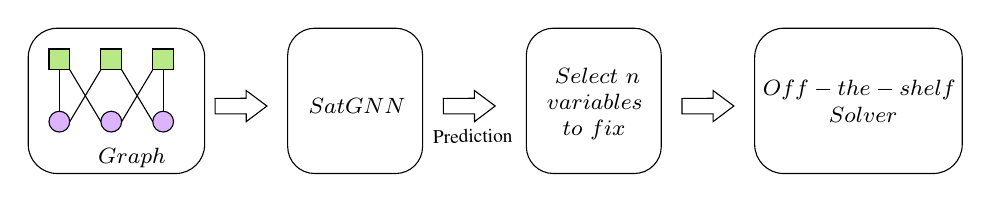
\begin{tikzpicture}[x=0.75pt,y=0.75pt,yscale=-1,xscale=1]
%uncomment if require: \path (0,451); %set diagram left start at 0, and has height of 451

%Shape: Rectangle [id:dp3587479777011455] 
\draw  [fill={rgb, 255:red, 184; green, 233; blue, 134 }  ,fill opacity=1 ] (75,295) -- (85,295) -- (85,305) -- (75,305) -- cycle ;
%Shape: Circle [id:dp623010589573948] 
\draw  [fill={rgb, 255:red, 144; green, 19; blue, 254 }  ,fill opacity=0.32 ] (100,330) .. controls (100,327.24) and (102.24,325) .. (105,325) .. controls (107.76,325) and (110,327.24) .. (110,330) .. controls (110,332.76) and (107.76,335) .. (105,335) .. controls (102.24,335) and (100,332.76) .. (100,330) -- cycle ;
%Shape: Circle [id:dp6210319224354044] 
\draw  [fill={rgb, 255:red, 144; green, 19; blue, 254 }  ,fill opacity=0.32 ] (125,330) .. controls (125,327.24) and (127.24,325) .. (130,325) .. controls (132.76,325) and (135,327.24) .. (135,330) .. controls (135,332.76) and (132.76,335) .. (130,335) .. controls (127.24,335) and (125,332.76) .. (125,330) -- cycle ;
%Shape: Circle [id:dp9356574928412065] 
\draw  [fill={rgb, 255:red, 144; green, 19; blue, 254 }  ,fill opacity=0.32 ] (75,330) .. controls (75,327.24) and (77.24,325) .. (80,325) .. controls (82.76,325) and (85,327.24) .. (85,330) .. controls (85,332.76) and (82.76,335) .. (80,335) .. controls (77.24,335) and (75,332.76) .. (75,330) -- cycle ;
%Shape: Rectangle [id:dp3734262207947956] 
\draw  [fill={rgb, 255:red, 184; green, 233; blue, 134 }  ,fill opacity=1 ] (100,295) -- (110,295) -- (110,305) -- (100,305) -- cycle ;
%Shape: Rectangle [id:dp01885589435556012] 
\draw  [fill={rgb, 255:red, 184; green, 233; blue, 134 }  ,fill opacity=1 ] (125,295) -- (135,295) -- (135,305) -- (125,305) -- cycle ;
%Straight Lines [id:da4907255353964277] 
\draw    (85,305) -- (100,330) ;
%Straight Lines [id:da9596012294566421] 
\draw    (130,305) -- (130,325) ;
%Straight Lines [id:da4248647563144248] 
\draw    (110,305) -- (125,330) ;
%Straight Lines [id:da6077808155610602] 
\draw    (110,330) -- (125,305) ;
%Straight Lines [id:da7849471865454107] 
\draw    (100,305) -- (85,330) ;
%Straight Lines [id:da019130866741998265] 
\draw    (80,305) -- (80,325) ;
%Down Arrow [id:dp06778528901825087] 
\draw   (170.04,330) -- (170.02,326.25) -- (155.03,326.29) -- (155.01,318.79) -- (170,318.75) -- (169.99,315) -- (180.01,322.47) -- cycle ;
%Rounded Rect [id:dp6272397850061886] 
\draw   (65,299) .. controls (65,291.27) and (71.27,285) .. (79,285) -- (136,285) .. controls (143.73,285) and (150,291.27) .. (150,299) -- (150,341) .. controls (150,348.73) and (143.73,355) .. (136,355) -- (79,355) .. controls (71.27,355) and (65,348.73) .. (65,341) -- cycle ;
%Rounded Rect [id:dp6283367026252633] 
\draw   (190,298) .. controls (190,290.82) and (195.82,285) .. (203,285) -- (242,285) .. controls (249.18,285) and (255,290.82) .. (255,298) -- (255,342) .. controls (255,349.18) and (249.18,355) .. (242,355) -- (203,355) .. controls (195.82,355) and (190,349.18) .. (190,342) -- cycle ;
%Rounded Rect [id:dp5504011516450884] 
\draw   (305,298) .. controls (305,290.82) and (310.82,285) .. (318,285) -- (357,285) .. controls (364.18,285) and (370,290.82) .. (370,298) -- (370,342) .. controls (370,349.18) and (364.18,355) .. (357,355) -- (318,355) .. controls (310.82,355) and (305,349.18) .. (305,342) -- cycle ;
%Rounded Rect [id:dp38041408857667824] 
\draw   (415,299) .. controls (415,291.27) and (421.27,285) .. (429,285) -- (501,285) .. controls (508.73,285) and (515,291.27) .. (515,299) -- (515,341) .. controls (515,348.73) and (508.73,355) .. (501,355) -- (429,355) .. controls (421.27,355) and (415,348.73) .. (415,341) -- cycle ;
%Down Arrow [id:dp2151743401001469] 
\draw   (280.01,330) -- (279.99,326.25) -- (265,326.29) -- (264.98,318.79) -- (279.97,318.75) -- (279.96,315) -- (289.98,322.47) -- cycle ;
%Down Arrow [id:dp19599668218528143] 
\draw   (394.99,330) -- (394.98,326.25) -- (379.99,326.29) -- (379.97,318.79) -- (394.96,318.75) -- (394.95,315) -- (404.96,322.47) -- cycle ;

% Text Node
\draw (258.63,332.91) node [anchor=north west][inner sep=0.75pt]  [rotate=-358.87] [align=left] {{\fontfamily{ptm}\selectfont {\scriptsize Prediction}}};
% Text Node
\draw (195,317.4) node [anchor=north west][inner sep=0.75pt]  [font=\footnotesize]  {$~SatGNN$};
% Text Node
\draw (71,341.4) node [anchor=north west][inner sep=0.75pt]  [font=\footnotesize]  {~~~~~~~$Graph$};
% Text Node
\draw (307,301.4) node [anchor=north west][inner sep=0.75pt]  [font=\footnotesize]  {$ \begin{array}{l}
\ Select\ n\ \\
variables\ \\
\ \ to\ fix
\end{array}$};
% Text Node
\draw (411,307.4) node [anchor=north west][inner sep=0.75pt]  [font=\footnotesize]  {$ \begin{array}{c}
Off-the-shelf\ \\
Solver
\end{array}$};


\end{tikzpicture}

}
\caption{Early fixing with SatGNN.}
\label{fig:ef-satgnn}
\end{figure}

Therefore, given a set $\hat{X}$ of random candidate solutions for a given problem instance, we compute \[
\hat{x}^* = \frac{1}{|\hat{X}|}\sum_{\hat{x}\in \hat{X}} \hat{x}\odot \hat{y}(\hat{x}) + (1-\hat{x}) \odot (1 - \hat{y}(\hat{x}))
,\] where $\odot$ is the element-wise product and $\hat{y}(\hat{x})$ is the predicted optimality of candidate solution $\hat{x}\in\hat{X}$ generated using the model from the previous experiment.
In the results reported 

Furthermore, we can say that the closer a given predicted optimal variable $\hat{x}^*_i$ is to 1 (resp. 0), the more certain the model is that that variable should be fixed at 1 (resp. 0).
Therefore, we use the model's certainty to select the variables to be fixed; that is, if we want to fix 50 binary variables, we will choose the 50 variables that the model is most certain of.
We evaluate the accuracy of the SatGNN for early fixing as a function of the number of fixed variables on the two instances of the test set.
These results can be seen in figure \ref{fig:ef-acc}.
As expected, the accuracy decreases as we include variables for which the model is less certain, to the limit of 82.5\% and 87.9\% accuracy on the two instances, which is the accuracy of the predicted optimal solution over the 1745 variables.
A summary of the model's performance when fixing all variables can be seen in Table \ref{tab:exp23-test-performance}.

\begin{figure}[!htb]
    \centering
    \includegraphics[width=0.4\textwidth]{figures/acc_97_9_6.png}
    \includegraphics[width=0.4\textwidth]{figures/acc_97_9_9.png}
    \caption{Early fixing accuracy for the two instances of the ONTS problem in the test set.}
    \label{fig:ef-acc}
\end{figure}

In face of these results, we evaluate how early fixing using SatGNN impacts the optimization performance both in terms of runtime and maximum objective value.
Specifically, we solve the two instances of the ONTS problem on the test set using Gurobi under an increasing number of fixed variables.
The results can be seen in figure \ref{fig:ef-impact}.

\begin{figure}[!htb]
    \centering
    \includegraphics[width=0.4\textwidth]{figures/runtime_obj_97_9_6.png}
    \includegraphics[width=0.4\textwidth]{figures/runtime_obj_97_9_9.png}
    \caption{Optimization results of the two ONTS instances with SatGNN-based early fixing. The objective is plotted with respect to the maximum of the original problem (without any fixed variables). Accuracy is measured with respect to the optimal value of the fixed variables.}
    \label{fig:ef-impact}
\end{figure}

As expected, correctly fixing the variables positively impacts the optimization, while wrongly fixing variables may decrease the runtime but often impacts the objective negatively.
However, we see that, at the limit, a substantial runtime reduction is achieved (90\% and 28\%, for instances 6 and 9, resp.) with a negligible objective cost (1.3\% and 0.3\%, resp.).
Beyond that, fixing more than 500 variables for instance 6 and more than 200 for instance 9 deemed the problems infeasible within a 5 minutes budget.

Given that the SatGNN model could generalize the optimality classification for larger instances of the problem, we also evaluate the impact of early fixing based on our model for the same two larger instances used in the previous experiment.
The performance on the larger instances can be seen in Figure \ref{fig:exp3-larger-instances} and in Table \ref{tab:exp23-test-performance}.
Even though these instances' sizes were not seen during training (not even during validation), the model was still able to handle them and provide sensible early fixing candidates.
The performance drop is significant in terms of accuracy and optimization performance.
In most configurations, however, the model was still able to reduce the runtime with little to no objective value reduction.

\begin{figure}[!htb]
    \centering
    \includegraphics[height=0.3\textwidth]{figures/acc_97_11.png}
    \includegraphics[height=0.3\textwidth]{figures/runtime_obj_97_11.png}
    \includegraphics[height=0.3\textwidth]{figures/acc_120_9.png}
    \includegraphics[height=0.3\textwidth]{figures/runtime_obj_120_9.png}
    \caption{Performance of SatGNN on early fixing instances larger than those seen during training and validation. Instance 97\_11 has 11 jobs, 2 more than the instances previously seen. Instance 120\_9 has the same amount of jobs but schedules for 120-time steps, 23 more than in the instances previously seen.}
    \label{fig:exp3-larger-instances}
\end{figure}

%\subsection{Discussion}

\section{Conclusion}
Throughout the paper, we first analyze the current evaluation methods for diffusion-based adversarial purification and then propose a recommendation for the reliable evaluation of the robustness of adversarial purification. We further investigate the influence of hyperparameters of the diffusion model on the robustness of the purification. Based on our analysis, we propose a new strategy to maximize the benefit of the purification methods.

\appendix
\section{Appendix for Proofs}

\paragraph{Proof of Theorem \ref{thm:main}.}

\begin{proof}
\label{proof:main}
Our proof has two steps. In Step 1, we will show that SimCLR is equivalent to minimizing the cross entropy loss defined in Eqn.~(\ref{eqn:cross-entropy}). 
In Step 2, we will show  that minimizing the cross-entropy loss 
is equivalent to spectral clustering on $\bfpi$. 
Combining the two steps together, we have proved our theorem. 

\textbf{Step 1: } SimCLR is equivalent to minimizing the cross entropy loss.

The cross-entropy loss takes expectation over 
$\bfW_\bfX\sim \mathbb{P}(\cdot ; \bfpi)$, 
which means $\bfW_\bfX$ has exactly one non-zero entry in each row $i$. By Lemma~\ref{lem:multinomial}, we know every row $i$ of $\bfW_\bfX$ is independent of other rows. Moreover, 
$\bfW_{\bfX,i}\sim \mathcal{M}(1, \bfpi_i/\sum_j \bfpi_{i,j})=\mathcal{M}(1, \bfpi_i)$, because $\bfpi_i$ itself is a probability distribution.
Similarly, we know $\bfW_\bfZ$ also has the row-independent property by sampling over $\mathbb{P}(\cdot;\bfK_\bfZ)$.
Therefore, by Lemma~\ref{lem:cross_split}, we know Eqn.~(\ref{eqn:cross-entropy}) is equivalent to:
\[
 -\sum_{i=1}^n \mathbb{E}_{\bfW_{\bfX,i}}[\log \mathbb{P}(\bfW_{\bfZ,i}=\bfW_{\bfX,i};\bfK_\bfZ)],
\]

This expression takes expectation over $\bfW_{\bfX,i}$ for the given row $i$. Notice that 
$\bfW_{\bfX,i}$ has exactly one non-zero entry, which equals $1$ (same for $\bfW_{\bfZ,i}$). 
As a result
we expand the above expression to be:
\begin{equation}
 -\sum_{i=1}^n \sum_{j\neq i} \Pr(\bfW_{\bfX,i,j}=1)\log \Pr(\bfW_{\bfZ,i,j}=1).
\label{eqn:detailed-expansion}    
\end{equation}


By Lemma~\ref{lem:multinomial}, $\Pr(\bfW_{\bfZ,i,j}=1)=\bfK_{\bfZ,i,j}/\|\bfK_{\bfZ,i}\|_1$ for $j\neq i$. Recall that $\bfK_\bfZ=(k(\bfZ_i-\bfZ_j))_{(i,j)\in[n]^2}$, which means 
$\bfK_{\bfZ,i,j}/\|\bfK_{\bfZ,i}\|_1=\frac{\exp(-\|\bfZ_i-\bfZ_j\|^2/{2\tau})}{\sum_{k\neq i}
\exp(-\|\bfZ_i-\bfZ_k\|^2/{2\tau})
}$ for $j\neq i$, when $k$ is the Gaussian kernel with variance $\tau$. 

Notice that $\bfZ_i=f(\bfX_i)$, so we know
\begin{equation}
-\log \Pr(\bfW_{\bfZ,i,j}=1)=
-\log \frac{\exp(-\|f(\bfX_i)-f(\bfX_j)\|^2/{2\tau})}{\sum_{k\neq i}
\exp(-\|f(\bfX_i)-f(\bfX_k)\|^2/{2\tau}),
}
\label{eqn:infonce-equivalence}    
\end{equation}


The right hand side is exactly the InfoNCE loss defined in Eqn.~(\ref{eqn:infonce}).
Inserting Eqn.~(\ref{eqn:infonce-equivalence}) into Eqn.~(\ref{eqn:detailed-expansion}), we get the SimCLR algorithm, which first samples augmentation pairs $(i,j)$ with $\Pr(\bfW_{\bfX,i,j}=1)$ for each row $i$, and then optimize the InfoNCE loss. 

\textbf{Step 2: } minimizing the cross entropy loss 
is equivalent to spectral clustering on $\bfpi$.


By Lemma~\ref{lem:convert_to_spectral}, we may further convert the loss to 
\begin{equation}
\label{eqn:main-theorem-repul-attr}
\min_{\bfZ}
-\sum_{(i,j)\in [n]^2} \mathbf{P}_{i,j}
\log k (\bfZ_i-\bfZ_j)+\log \mathbf{R}(\bfZ).
\end{equation}
Since $k$ is the Gaussian kernel, this reduces to \[
\min_\bfZ \mathrm{tr}(\bfZ^\top \mathbf{L}(\bfpi) \bfZ)
+\log \mathbf{R}(\bfZ),
\]

where we use the fact that $\mathbb{E}_{\bfW_\bfX\sim \mathbb{P}(\cdot; \bfpi)}[\mathbf{L}(\bfW_\bfX)]
=\mathbf{L}(\bfpi)
$, because the Laplacian operator is linear and $
\mathbb{E}_{\bfW_\bfX\sim \mathbb{P}(\cdot; \bfpi)}(\bfW_\bfX)=\bfpi
$.
\end{proof}

\paragraph{Proof of Theorem \ref{thm:clip}.}
\begin{proof}
Since $\bfW_\bfX\sim \mathbb{P}(\cdot;\bfpi_{\mathbf{A}, \mathbf{B}})$, we know 
$\bfW_\bfX$ has exactly one non-zero entry in each row, denoting the pair that got sampled. 
A notable difference compared to the previous proof is we now have $n_\mathcal{A}+n_\mathcal{B}$ objects in our graph. CLIP deals with this by taking a mini-batch of size $2N$, 
such that $n_\mathcal{A}=n_\mathcal{B}=N$, and adding the $2N$ InfoNCE losses together. We label the objects in $\mathcal{A}$ as $[n_\mathcal{A}]$, and the objects in $\mathcal{B}$ as $\{n_\mathcal{A}+1, \cdots, n_\mathcal{A}+n_\mathcal{B}\}$. 

Notice that $\bfpi_{\mathbf{A}, \mathbf{B}}$ is a bipartite graph, so the edges of objects in $\mathcal{A}$ will only connect to object in $\mathcal{B}$ and vice versa. We can define the similarity matrix in $\cZ$ as $\bfK_\bfZ$, 
where $\bfK_\bfZ(i, j+n_\mathcal{A})=\bfK_\bfZ(j+n_\mathcal{A},i)= k(\bfZ_i-\bfZ_j)$ for $i\in [n_\mathcal{A}], j\in [n_\mathcal{B}]$, and otherwise we set $\bfK_\bfZ(i,j)=0$. 
The rest is same as the previous proof. 
\end{proof}

\paragraph{Proof of Theorem \ref{thm:exponential}.}

\begin{proof}
\label{proof:exponential}
Since the objective function consists of a linear term combined with an entropy regularization, which is a strongly concave function, the maximization problem is a convex optimization problem. Owing to the implicit constraints provided by the entropy function, the problem is equivalent to having only the equality constraint. We then introduce the Lagrangian multiplier $\lambda$ and obtain the following relaxed problem:

$$
\widetilde{E}(\boldsymbol{\alpha})=\psi_{1}-\sum_{i=1}^n \alpha_{i} \psi_{i}+\tau \sum_{i=1}^n \alpha_{i}\log \alpha_{i}+\lambda\left(\boldsymbol{\alpha}^{\top} \mathbf{1}_n-1\right).
$$

As the relaxed problem is unconstrained, taking the derivative with respect to $\alpha_{i}$ yields

$$
\frac{\partial \widetilde{E}(\boldsymbol{\alpha})}{\partial \alpha_{i}}=-\psi_{i}+\tau\left(\log \alpha_{i}+\alpha_{i} \frac{1}{\alpha_{i}}\right)+\lambda=0.
$$

Solving the above equation implies that $\alpha_{i}$ takes the form
$
\alpha_{i}=\exp \left(\frac{1}{\tau} \psi_{i}\right) \exp \left(\frac{-\lambda}{\tau}-1\right).
$ Since $\alpha_{i}$ lies on the probability simplex, the optimal $\alpha_{i}$ is explicitly given by
$
\alpha^{*}_{i}=\frac{\exp \left(\frac{1}{\tau} \psi_{i}\right)}{\sum_{i^{\prime}=1}^n \exp \left(\frac{1}{\tau} \psi_{i^{\prime}}\right)} .
$ Substituting the optimal point into the objective function, we obtain
$$
\begin{aligned}
E\left(\boldsymbol{\alpha}^*\right)  &=\psi_1-\sum_{i=1}^n \frac{\exp \left(\frac{1}{\tau} \psi_{i}\right)}{\sum_{i^{\prime}=1}^n \exp \left(\frac{1}{\tau} \psi_{i^{\prime}}\right)} \psi_{i}+\tau \sum_{i=1}^n \frac{\exp \left(\frac{1}{\tau} \psi_{i}\right)}{\sum_{i^{\prime}=1}^n \exp \left(\frac{1}{\tau} \psi_{i^{\prime}}\right)}\log \frac{\exp \left(\frac{1}{\tau} \psi_{i}\right)}{\sum_{i^{\prime}=1}^n \exp \left(\frac{1}{\tau} \psi_{i^{\prime}}\right)} \\
& =\psi_1 - \tau \log \left(\sum_{i=1}^n \exp \left(\frac{1}{\tau} \psi_{i}\right)\right).
\end{aligned}
$$
Thus, the Lagrangian dual function is given by
\begin{equation*}
-E\left(\boldsymbol{\alpha}^*\right)= -\tau \log \frac{\exp \left(\frac{1}{\tau} \psi_{1}\right)}{\sum_{i=1}^n \exp \left(\frac{1}{\tau} \psi_{i}\right)}.\qedhere
\end{equation*}
\end{proof}



\section{More on Experiments} \label{section: experiment_details}

\paragraph{CIFAR-10 and CIFAR-100} CIFAR-10 ~\citep{krizhevsky2009learning} and CIFAR-100 ~\citep{krizhevsky2009learning} are well-known classic image classification datasets. Both CIFAR-10 and CIFAR-100 contain a total of 60k $32 \times 32$ labeled images of different classes, with 50k for training and 10k for testing. CIFAR-10 is similar to CIFAR-100, except there are 10 different classes in CIFAR-10 and 100 classes in CIFAR-100.

\paragraph{TinyImageNet} TinyImageNet ~\citep{le2015tiny} is a subset of ImageNet ~\citep{deng2009imagenet}. There are 200 different object classes in TinyImageNet, with 500 training images, 50 validation images, and 50 test images for each class. All the images in TinyImageNet are colored and labeled with a size of $64 \times 64$.

\textbf{Pseudo-code.} Algorithm \ref{alg:Training Procedure} presents the pseudo-code for our empirical training procedure.

\begin{algorithm}[!htbp]
\caption{Training Procedure}
\label{alg:Training Procedure}
\begin{algorithmic}[1]
\REQUIRE trainable encoder network $f$, batch size $N$, augmentation strategy \textit{aug}, loss function $L$ with hyperparameters \textit{args}
\FOR {sampled minibatch ${x_i}_{i=1}^N$}
\FORALL{$i \in { 1, ..., N }$}
\STATE draw two augmentations $t_i = \textit{aug}\left(x_i\right) $, $t_i' = \textit{aug}\left(x_i\right) $
\STATE $z_i = f\left(t_i\right)$, $z_i' = f\left(t_i'\right)$
\ENDFOR
\STATE compute loss $\mathcal{L} = L(N, z, z', \textit{args})$
\STATE update encoder network $f$ to minimize $\mathcal{L}$
\ENDFOR
\STATE \textbf{Return} encoder network $f$
\end{algorithmic}
\end{algorithm}

We also provide the pseudo-code for our core loss function used in the training procedure in Algorithm \ref{alg:Core loss}. The pseudo-code is almost identical to SimCLR's loss function, with the exception of an extra parameter $\gamma$.

\begin{algorithm}[!htbp]
\caption{Core loss function $\mathcal{C}$}
\label{alg:Core loss}
\begin{algorithmic}[1]
\REQUIRE batch size $N$, two encoded minibatches $z_1, z_2$, $\gamma$, temperature $\tau$
\STATE $z = \textit{concat}\left(z_1, z_2\right)$
\FOR {$i \in {1, ..., 2N }, j \in {1, ..., 2N}$ }
\STATE $s_{i,j} = \Vert z_i - z_j \Vert_2^{\gamma}$
\ENDFOR
\STATE \textbf{define} $l(i, j)$ \textbf{as} $l(i, j) = - \log \frac{exp\left(s_{i,j}/\tau \right)}{\sum_{k=1}^{2N} \mathbf{1}{[k \ne i]} exp\left(s{i, j} / \tau \right)} $
\STATE \textbf{Return} $\frac{1}{2N} \sum_{k=1}^N\left[l(i, i+N) + l(i+N, i)\right]$
\end{algorithmic}
\end{algorithm}

Utilizing the core loss function $\mathcal{C}$, we can define all kernel loss functions used in our experiments in Table \ref{table: loss definition}. For all $z_i \in z$ with even dimensions $n$, we define $z_{L_i} = z_i\left[0:n/2\right]$ and $z_{R_i} = z_i\left[n/2:n\right]$.

\begin{table}[ht]
\centering
\begin{tabular}{{@{}l|l@{}}}
Kernel  &  Loss function \\ \midrule
Laplacian & $\mathcal{C}\left(N, z, z', \gamma=1, \tau\right)$\\ \midrule
Sum       & $\lambda * \mathcal{C}\left(N, z, z', \gamma=1, \tau_1\right) + (1-\lambda) * \mathcal{C}\left(N, z, z', \gamma=2, \tau_2\right)$  \\ \midrule
Concatenation Sum&$\lambda * \mathcal{C}\left(N, z_L, z'_L, \gamma=1, \tau_1\right) + (1-\lambda) * \mathcal{C}\left(N, z_R, z'_R, \gamma=2, \tau_2\right)$\\ \midrule
$\gamma = 0.5$ & $\mathcal{C}\left(N, z, z', \gamma=0.5, \tau\right)$          \\ 

\end{tabular}

\caption{Definition of kernel loss functions in our experiments}
\label {table: loss definition}
\end{table}

\textbf{Baselines.} We reproduce the SimCLR algorithm using PyTorch Lightning~\citep{PytorchLightning}.

\textbf{Encoder details.}
The encoder $f$ consists of a backbone network and a projection network. We employ ResNet50~\citep{ResNet} as the backbone and a 2-layer MLP (connected by a batch normalization~\citep{ioffe2015batch} layer and a ReLU \cite{nair2010rectified} layer) with hidden dimensions 2048 and output dimensions 128 (or 256 in the concatenation kernel case).

\textbf{Encoder hyperparameter tuning.}
For each encoder training case, we randomly sample 500 hyperparameter groups (sample details are shown in Table \ref{table: Hyperparameter sample}) and train these samples simultaneously using Ray Tune ~\citep{RayTune}, with the ASHA scheduler~\citep{li2018massively}. Ultimately, the hyperparameter group that maximizes the online validation accuracy (integrated in PyTorch Lightning) within 5000 validation steps is chosen for the given encoder training case.

\begin{table}[ht]
\centering

\begin{tabular}{@{}l|l|l@{}}
\midrule
Hyperparameter  & Sample Range & Sample Strategy \\ \midrule
start learning rate & $\left[10^{-2}, 10\right]$ & log uniform \\ \midrule
$\lambda$       & $\left[0, 1\right]$ & uniform \\ \midrule
$\tau$, $\tau_1$, $\tau_2$ & $\left[0, 1\right]$ & log uniform \\ \midrule
\end{tabular}

\caption{Hyperparameters sample strategy}
\label {table: Hyperparameter sample}
\end{table}

\textbf{Encoder training.} 
We train each encoder using the LARS optimizer~\citep{LARSOptimizer}, LambdaLR Scheduler in PyTorch, momentum 0.9, weight decay $10^{-6}$, batch size 256, and the aforementioned hyperparameters for 400 epochs on a single A-100 GPU.

\textbf{Image transformation.} The image transformation strategy, including augmentation, is identical to the default transformation strategy provided by PyTorch Lightning.

\textbf{Linear evaluation.}
The linear head is trained using the SGD optimizer with a cosine learning rate scheduler, batch size 64, and weight decay $10^{-6}$ for 100 epochs. The learning rate starts at $0.3$ and ends at $0$.

\textbf{Moco Experiments.} We also tested our method based on MoCo~\citep{he2019moco}. The results are summarized in Table \ref{tab:results-moco}. Here we choose ResNet18~\citep{ResNet} as the backbone and set a temperature of $0.1$ as default. For our simple sum kernel, we set $\lambda=0.8$. The results show that our method outperforms the original MoCo method.

\begin{table}[thb]
\centering
\caption{MoCo Experiment Results on CIFAR-10 and CIFAR-100.}
\label{tab:results-moco}
\resizebox{\textwidth}{!}{%
\begin{tabular}{@{}c|ccc|ccc@{}}
\toprule
\multirow{3}{*}{Method} & \multicolumn{3}{c|}{CIFAR-10} & \multicolumn{3}{c}{CIFAR-100} \\ \cmidrule(lr){2-4} \cmidrule(lr){5-7} 
                        & 200 epochs & 400 epochs    & 1000 epochs   & 200 epochs & 400 epochs & 1000 epochs         \\ \midrule
MoCo (repro.)         & $76.41 \pm 0.12$    & $80.01 \pm 0.15$          & $84.45 \pm 0.08$    & $\mathbf{47.02 \pm 0.11}$ & $52.50 \pm 0.07$ & $57.62 \pm 0.15$            \\
\midrule
Laplacian Kernel        & ${78.09 \pm 0.10}$    & $\mathbf{83.85 \pm 0.09}$          & $\mathbf{88.34 \pm 0.16}$    & $46.12 \pm 0.22$   & $53.44 \pm 0.17$ & $59.10 \pm 0.14$        \\
Simple Sum Kernel & $\mathbf{78.12 \pm 0.15}$   & $83.23 \pm 0.18$ & $87.50 \pm 0.20$ & $46.65 \pm 0.06$ & $\mathbf{53.62 \pm 0.19}$ & $\mathbf{59.83 \pm 0.12}$\\
\bottomrule
\end{tabular}
}
\end{table}



\section{More Experiments on Synthetic Data}


Consider a scenario with $n$ clusters, each containing $k$ vertices. Let the probability of vertices $u$ and $v$ from the same cluster belonging to $\bfpi$ be $p$. Conversely, for vertices $u$ and $v$ from different clusters, let the probability of belonging to $\pi$ be $q$. We generate the graph $\bfpi$ randomly, based on $p$ and $q$. We experiment with values of $k=100$ and $n=6$ for ease of visualization, embedding all points in a two-dimensional space. Each vertex's initial position originates from a normal distribution. In each iteration, we sample a subgraph of $\bfpi$ uniformly, ensuring each vertex has an out-degree of $1$. We then optimize the corresponding vectors using InfoNCE loss with an SGD optimizer and iterate until convergence. Our experimental setup consists of an SGD learning rate of $1$, an InfoNCE loss temperature of $0.5$, and a batch size of $50$. We evaluate two scenarios with different $p$ and $q$ values: $p=1$, $q=0$, and $p=0.75$, $q=0.2$. The results of these experiments are visualized in Figure \ref{fig:vis-spectral-cluster}. The obtained embeddings exhibit the hallmark pattern of spectral clustering of graph $\bfpi$.

\begin{figure}[!tb]
\centering
\subfigure{
\includegraphics[width=1\textwidth]{Figures/cluster_pi.png}
\label{fig:vis-cluster}
}
\subfigure{
\includegraphics[width=1\textwidth]{Figures/noised_cluster_pi.png}
\label{fig:vis-noised-cluster}
}
\caption{Visualizations of the optimization process using InfoNCE Loss on the vectors corresponding to $\bfpi$. Points of identical color belong to the same cluster within $\bfpi$. To showcase the internal structure of $\bfpi$, we randomly select 10 vertices from each cluster to display the edge distribution of $\bfpi$.}
\label{fig:vis-spectral-cluster}
\end{figure}



\printbibliography
% \bibliography{bibliography}

\balance

\end{document}
